\documentclass[a4paper,12pt]{article}

%%% Работа с русским языком
\usepackage{cmap}					% поиск в PDF
\usepackage{mathtext} 				% русские буквы в формулах
\usepackage[T2A]{fontenc}			% кодировка
\usepackage[utf8]{inputenc}			% кодировка исходного текста
\usepackage[english,russian]{babel}	% локализация и переносы
\usepackage[table,xcdraw]{xcolor}
%%% Дополнительная работа с математикой
\usepackage{amsfonts,amssymb,amsthm,mathtools} % AMS
\usepackage{amsmath}
\usepackage{icomma} % "Умная" запятая: $0,2$ --- число, $0, 2$ --- перечисление

\usepackage[left = 2cm, right = 2cm, top = 2cm, bottom = 2cm]{geometry}

\usepackage{graphicx}

%% Номера формул
%\mathtoolsset{showonlyrefs=true} % Показывать номера только у тех формул, на которые есть \eqref{} в тексте.

%% Шрифты
\usepackage{euscript}	 % Шрифт Евклид
\usepackage{mathrsfs} % Красивый матшрифт

%% Свои команды
\DeclareMathOperator{\sgn}{\mathop{sgn}}

%% Перенос знаков в формулах (по Львовскому)
\newcommand*{\hm}[1]{#1\nobreak\discretionary{}
	{\hbox{$\mathsurround=0pt #1$}}{}}

%%% Работа с картинками
\usepackage{graphicx}  % Для вставки рисунков
\graphicspath{{images/}{images2/}}  % папки с картинками
\setlength\fboxsep{3pt} % Отступ рамки \fbox{} от рисунка
\setlength\fboxrule{1pt} % Толщина линий рамки \fbox{}
\usepackage{wrapfig} % Обтекание рисунков и таблиц текстом

%%% Работа с таблицами
\usepackage{array,tabularx,tabulary,booktabs} % Дополнительная работа с таблицами
\usepackage{longtable}  % Длинные таблицы
\usepackage{multirow} % Слияние строк в таблице
\usepackage{upgreek}
\usepackage{enumerate}
\usepackage{ dsfont }
\usepackage[weather]{ifsym}

%%% Цветной текст

\usepackage{movie15}
% in preamble
\usepackage{graphicx}
\usepackage{animate}


\usepackage{colortbl}

%%% Гиперссылки

\usepackage{xcolor}
\usepackage{hyperref}
\definecolor{linkcolor}{HTML}{199B03} % цвет ссылок
\definecolor{urlcolor}{HTML}{199B03} % цвет гиперссылок

\hypersetup{pdfstartview=FitH,  linkcolor=linkcolor,urlcolor=urlcolor, colorlinks=true}

%%% Tikz

\usepackage{tikz}
\usetikzlibrary{shapes.geometric, arrows}
\tikzstyle{startstop} = [ellipse, minimum width=5cm, minimum height=2cm,text centered, draw=black, fill=blue!40]

\tikzstyle{medium} =[rectangle, rounded corners, minimum width=5cm, minimum height=2cm,text centered, draw=black, fill=green!40]

\tikzstyle{test} =[rectangle, rounded corners, minimum width=5cm, minimum height=2cm,text centered, draw=black, fill=orange!40]


\tikzstyle{alg} = [circle, minimum width=2cm, minimum height=2cm, text centered, draw=black, fill=green!30]

\tikzstyle{rforest} = [diamond, minimum width=3cm, minimum height=1cm, text centered, draw=black, fill=green!30]

%\tikzstyle{arrow} = [thick,->,>=stealth]
\tikzset{arw/.style={-triangle 60,line width=1pt,shorten <= 4pt}}


%%% Заголовок
\author{Зехов Матвей}
\title{Курсовая работа}
\date{\today}

\begin{document}
	
	
\thispagestyle{empty}
\begin{center}
	\textbf{ПРАВИТЕЛЬСТВО РОССИЙСКОЙ ФЕДЕРАЦИИ}\\
	\vspace{2ex}
	\textbf{Федеральное государственное автономное\\ образовательное учреждение высшего образования}
	
	\vspace{2ex}
	
	\textbf{Национальный исследовательский университет \\ <<Высшая школа экономики>>}
	
	\vspace{8ex}
	\begin{flushright}
		Факультет экономических наук\\
		Образовательная программа <<Экономика>>
	\end{flushright}
\end{center}
\vspace{9ex}

\begin{center}
	{\textbf{КУРСОВАЯ РАБОТА
	}}
	\vspace{1ex}
	
	<<Принцип мета-обучения для отбора моделей при прогнозировании одномерных временных рядов>>
\end{center}
\vspace{1ex}
\begin{flushright}
	\noindent
	Студент группы БЭК162\\Зехов Матвей Сергеевич\\
	\vspace{13ex}
	Научный руководитель:\\
	Демешев Борис Борисович
	
\end{flushright}	

\vfill

\begin{center}
	Москва 2019
	
\end{center}

\newpage

\tableofcontents
	
\newpage

\section{Введение}

Качественное прогнозирование временных рядов  -- это процесс, требующий порой больших затрат времени и интеллектуальных ресурсов. Однако в рамках современных условий необходимого времени на тщательный отбор модели может попросту не быть. Например, если рядов большое количество, а обучать несколько моделей на каждом из них слишком долго. 

Принцип мета-обучения предлагает решение проблемы отбора моделей. Основная идея подхода описана в \cite{start}, \cite{pca}, \cite{meta} и заключается в отборе моделей не на основе, например, наименьшей ошибки напрямую, а исходя из специфических характеристик временного ряда, которые можно вычислить быстро. Если говорить более общими словами, подход мета-обучения в данном контексте подразумевает переход к решению классической задачи классификации в машинном обучении. 


\begin{figure}[!h]
	\begin{center}
		\resizebox{0.8\textwidth}{!}{%
			\begin{tikzpicture}[node distance=2cm]
			\node (start) [startstop] {Временные ряды};
			\node (dat) [medium, below of=start, yshift=-1cm] {Наблюдаемые ряды};
			\node (sim) [medium, right of = dat, xshift = 6cm] {Симуляции};
			\node (test) [test, right of = start, xshift = 17cm] {Новые  ряды};
			\node (feat_new) [test, below of = test, yshift = -1.5cm, text width = 6cm] {Вычисление характеристик};
			\node (full) [medium, below of = dat, yshift = -1cm] {Выборка};
			\node (tr) [medium, below of = full, yshift = -1cm, text width = 5cm]
			{Тренировочная часть};
			\node (ts) [medium, right of = tr, xshift = 13cm] {Тестовая часть};
			\node (feat) [medium, below of = tr, yshift = -1cm, text width = 6cm] {Вычисление характеристик};
			\node (fit) [medium, right of = feat, xshift = 5.5cm,  text width = 5cm]
			{Обучение моделей};
			\node (best) [medium, below of = ts, yshift = -1.5cm, text width = 5cm]
			{Выбор лучшей модели};
			\node (labs) [medium, below of = best, yshift = -1.5cm, text width = 5cm]
			{Выделение лейблов};
			\node (al) [alg, below of = feat, yshift = -4cm, text width = 6cm]{Обучение классификатора};
			\node (rf) [rforest, below of = fit, yshift = -10cm, text width = 4cm]{Случайный лес};
			\node (forec) [test, below of = rf, yshift = -3.5cm, text width = 5cm]{Предсказание};
			
			
			\draw [arw] (start) -- (dat);
			\draw [arw] (start) -- (test);
			\draw [arw] (dat) -- (sim);
			\draw [arw] (sim) -- (full);
			\draw [arw] (dat) -- (full);
			\draw [arw] (full) -- (tr);
			\draw [arw] (full) -- (ts);
			\draw [arw] (tr) -- (fit);
			\draw [arw] (feat) -- (al);
			\draw [arw] (tr) -- (feat);
			\draw [arw] (ts) -- (best);
			\draw [arw] (best) -- (labs);
			\draw [arw] (fit) -- (best);
			\draw [arw] (al) |- (rf);
			\draw [arw] (labs) |- (al);
			\draw [arw] (test) -- (feat_new);
			\draw [arw] (feat_new) |- (rf);
			\draw [arw] (rf) -- (forec);
			
			
			\end{tikzpicture}
			%
		}
		
	\end{center}
	\label{tikz}
	\caption{Алгоритм мета-обучения}
\end{figure}


Разберём подход пошагово. Для наглядности схему алгоритма можно увидеть на Рис.~\ref{tikz}. Предположим, что в нашем распоряжении имеется выборка из временных рядов достаточного размера, сформирован некоторый пул моделей, из которого будет производиться выбор, а также известен список характеристик временных рядов.

\begin{enumerate}
	\item Сформируем некоторое множество рядов, которое будет нашей выборкой. 
	
	\item Сгенерируем на основе выборки некоторое количество симулированных рядов для расширения признакового богатства выборки. Добавим их в основную выборку.
	
	\item Каждый ряд новой выборки разделим на тренировочную и тестовую части.
	
	\item На основе тренировочной части вычислим вектор характеристик. Набор таких векторов и будет мета-данными.
	
	\item На основе тренировочной части обучим каждую модель из пула моделей. На основе каждой модели построим прогноз соответственно длине тестовой части ряда и вычислим ошибки. Прогноз будет строиться без переоценки модели, лишь с увеличением горизонта. На основе наименьшей ошибки присвоим ряду лейбл в виде названия модели. 
	
	\item Получив на основе разметки рядов матрицу характеристик и вектор лейблов, получим набор данных каноничного вида, пригоднный для обработки любого мультиклассового классификатора. 
	
	\item Обучим классификатор. Например, неплохо подойдёт случайный лес. Такой подход использовался в \cite{start}. Существует также пример с нейросетью в \cite{neural}.
	
	\item Для построения прогноза на новых рядах необходимо вычислить их характеристики и построить на них прогноз предобученного случайного леса.
	
	
\end{enumerate}

Последующие главы данной работы будут нацелены на подробный разбор всех вышеперечисленных шагов. 




\newpage
\section{Предварительная обработка данных}

Данные для данной работы взяты из датасета соревнования M4. Он содержит $ 100 000 $ временных рядов различной длины. Данные не размечены по принадлежности (макроэкономика, демография и т.д.), поэтому от попыток их интерпретировать можно смело абстрагироваться. 

В качестве первого этапа сформируем необходимую выборку и преобразуем данные. Рассмотрим каждый класс рядов, сгруппированных по периодичности. В нашем распоряжении годовые, квартальные, месячные, недельные, дневные и почасовые данные. Первое, что попытаемся учесть, это сбалансированность классов. То есть попытаемся брать одинаковые размеры выборки. Изначально предполагалось взять по две тысячи рядов каждой группы, однако это оказалось затруднительно по причине, изложенной ниже. 

Так как все ряды имеют различные длины, было решено унифицировать длину ряда в каждой группе. Для этого в каждом кластере была определена фиксированная длина ряда. Далее из исходных данных удалялись все ряды короче этой длины. На следующем шаге из оставшихся данных случайным образом без возвращения выбирались 2000 рядов. Если ряд был длиннее фиксированной длины, то он обрезался. Однако оказалось, что недельных и почасовых рядов после фильтрации осталось очень мало, поэтому эти кластеры были включены целиком. 

Параметры выборки представлены в следующей таблице:

\begin{center}
\begin{tabular}{|
		>{\columncolor[HTML]{91FF91}}l |l|l|l|}
	\hline
	\textbf{Класс} & \cellcolor[HTML]{91FF91}\textbf{\begin{tabular}[c]{@{}l@{}}Количество\\ в выборке\end{tabular}} & \cellcolor[HTML]{91FF91}\textbf{Длина ряда} & \cellcolor[HTML]{91FF91}\textbf{\begin{tabular}[c]{@{}l@{}}Период\\ сезонности\end{tabular}} \\ \hline
	\textbf{Yearly} & 2000 & 30 & 1 \\ \hline
	\textbf{Quarterly} & 2000 & 60 & 4 \\ \hline
	\textbf{Monthly} & 2000 & 156 & 12 \\ \hline
	\textbf{Weekly} & 286 & 315 & 4 \\ \hline
	\textbf{Daily} & 2000 & 500 & 7 \\ \hline
	\textbf{Hourly} & 245 & 720 & 24 \\ \hline
	\textbf{Total} & 8531 &  &  \\ \hline
\end{tabular}

\end{center}

В итоге мы получили выборку из 8531 временных рядов, сгруппированных по периодичности и длине. Так как характеристики рядов не должны зависеть от шкалы ряда \cite[cтр.~4]{start}, их необходимо центрировать и нормировать. Для этого просто вычтем из каждого значения среднее и поделим на корень из выборочной дисперсии:

\[ \tilde{X_i} = \frac{X_i - \bar{X}}{\hat{\sigma}} \quad \hat{\sigma}^2 =  \frac{\sum_{1}^{n} (X_i - \bar{X})^2}{n - 1}  \]

В результате на графиках на Рис. \ref{examples} можно увидеть примеры стандартизированных рядов из выборки.
\begin{figure}[h]
	
	\centering
	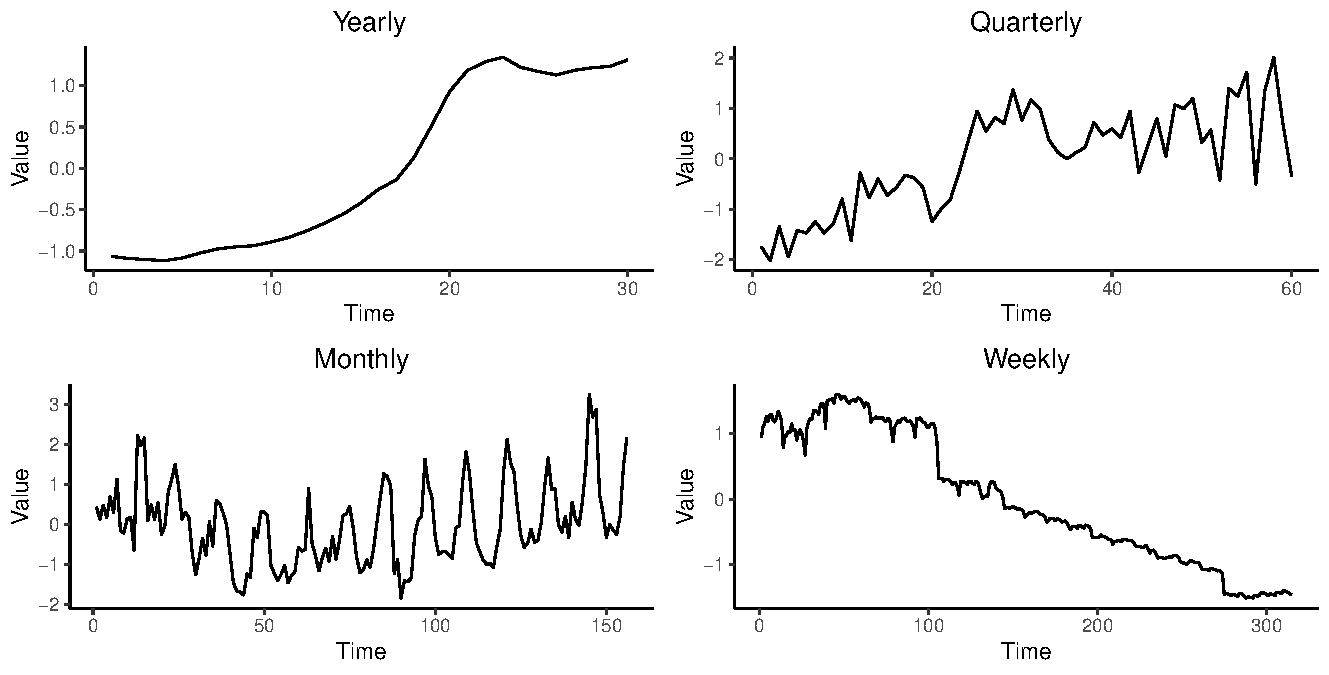
\includegraphics[width=1\linewidth]{time_series}
	
	
	\caption{Стандартизированные временные ряды}
	\label{examples}
\end{figure}
	
Важно сделать небольшое замечание. Перед стандартизацией необходимо проверить выборку на наличие константных рядов. В данной реализации выборки нашёлся только один такой годовой ряд, и он был удалён. Если этого не сделать, но при нормировке произойдёт деление на ноль и ряд превратится в последовательность пропущенных значений. Следовательно, в итоге осталось 8530 временных рядов.
	

\newpage
\section{Характеристики временных рядов}

Теперь, после предварительной обработки данных, необходимо рассчитать характеристики временных рядов. Всего для каждого ряда были вычислены 23 характеристики. \cite{start}

\begin{enumerate}
	\item Автокорреляционные характеристики:
		\begin{enumerate}
			\item Автокорреляция первого порядка. 
			\item Автокорреляция первого порядка после взятия разностей.
			\item Автокорреляция первого порядка после двукратного взятия разностей.
			\item Частная автокорреляция пятого порядка.
		\end{enumerate}
	
	\item Спектральная энтропия (Shannon entropy)
	\[ H = - \int_{-\pi}^{\pi}\hat{f}(\lambda) \log(\hat{f}(\lambda)) d\lambda \]
	
	Спектральная энтропия вычисляется как обычная энтропия в непрерывном случае, однако в место функции плотности используется оценка спектральной плотности. Оценку этой функции можно получить из преобразования Фурье. Данный признак позволяет оценивать склонность ряда к прогнозированию. Относительно малое значение говорит о том, что временной ряд содержит сильный сигнал и что его легче прогнозировать, относительно большое -- о том, что он содержит в себе больше неопределённости и, соответственно, что его сложнее будет прогнозировать. 
	
	\item Lumpiness and stability
	
	
	Две данные характеристики взаимосвязаны между собой. Для их подсчёта временной ряд делится на несколько непересекающихся окон. Если данные сезонные, то ширина окна равна периодичности. В ином случае ширина окна равна 10. Далее для каждого отрезка вычисляются выборочное среднее и выборочная дисперсия. 
	
	Stability -- это выборочная дисперсия выборочных средних, а Lumpiness -- это выборочная дисперсия выборочных дисперсий. \cite{anomalous}
	
	\item Crossing points
	
	Данная характеристика обозначает количество пересечений временного ряда с линией медианы ряда.
	
	\item Показатель Хёрста (Hurst)
	
	Для измерения степени долгосрочной памяти процесса будем использовать следующую характеристику: 0.5 + оценка метода максимального правдоподобия параметра частичного дифференцирования $ d $, описанного в \cite{frac}. Параметр частичного дифференцирования характеризует класс моделей с долгосрочной памятью. Например, в авторегрессионных моделях с частичным дифференцированием автокорреляция убывает с ростом лага не экспоненциально, а медленнее, по степенной функции. Поэтому такие процессы сохраняют зависимость от более глубоких лагов.  \cite[стр.~19]{meta}
	
	\item Unitroot KPSS
	
	Статистика для KPSS-теста о стационарности временного ряда. 
	
	\item Нелинейность 
	
	Коэффициент нелинейности вычислялся с помощью модифицированного теста Teräsvirta \cite{nonlin}. Этот тест использует статистику вида $ \chi^2  = T ln(RSS_1/RSS_2) $, где $ RSS_1 $ и $ RSS_2 $ это суммы квадратов остатков в нелинейной и линейной авторегрессиях соответственно. Текущая модификация считает статистику $ \frac{10 \chi^2}{T} $, которая сходится к значению, характеризующему степень нелинейности при $ T \to \infty $, где $ T $ является длиной ряда. Большое значение означает высокую нелинейность, маленькое - низкую.
	
	\item Excess Kurtosis
	
	Куртозис является ни чем иным, как стандартизированым четвёртым центральным моментом. В нашем случае, выборочным. Для любого нормального распределения куртозис всегда равняется 3, поэтому в качестве характеристики обычно считают избыточный куртозис:
	
	\[ \hat{\text{Kurt}}(X) =\frac{\frac{1}{n} \sum_T (X_i - \bar{X})^4}{(\frac{1}{n} \sum_T (X_i - \bar{X})^2)^2}  - 3 \]
	
	\item Скошенность (Skewness)
	
	Скошенность распределения характеризуется его стандартизированным третьим центральным моментом. Аналогично, он будет выборочным. 
	
	\[ 	\hat{\text{Skew}}(X) =\frac{\frac{1}{n} \sum_T (X_i - \bar{X})^3}{ \left(\sqrt{\frac{1}{n} \sum_T (X_i - \bar{X})^2} \right)^2} \]
	
	\item Хаос
	
	Степень хаотичности системы вычисляется по специальному методу, описанному в красочной и весьма занимательной статье \cite{chaos}.  Идейно этот подход похож на метод поиска экспоненты Ляпунова, однако суть несколько иная. Данная работа не подразумевает подробного обзора этого метода, поэтому он будет опущен. Итоговое значение теста ранжируется на отрезке $ [0, 1] $. Ноль означает регулярную систему, тогда как единица - хаотическую. 
	
	\item Изменение уровня (Level shift)
	
	Изменение уровня вычисляется как максимальное изменение выборочного среднего по сдвигающемуся окну. Размер окна устанавливался равным периодичности сезонных данных, а для годовых данных был равен десяти. 
	
	\item Плоские пятна (Flat spots)
	
	Данная характеристика вычисляется путём деления области значения временного ряда на десять равных отрезков и определения максимальной длины участка, укладывающегося в один интервал.
	
	\item Максимальное расстояние Кульбака-Лейблера (Max KL-divergence)
	
	Данная статистика вычисляет максимальное расстояние Кульбака-Лейблера между двумя последовательными пересекающимися блоками (сдвигающееся окно). Ширина окна как и ранее равна периодичности данных, либо 10 для годовых данных.
	
	\item Коэффициент формы экстремального распределения (Extreme distribution shape parameter)
	
Эта характеристика вычисляется с помощью оценки параметра формы обобщённого экстремального распределения (GEV), то есть распределения граничных порядковых статистик. Обозначим этот параметр за $ \xi $. Обычно выделяются три типа распределений в зависимости от значения этого параметра. Их можно увидеть на графике на Рис. \ref{gev}\footnote{График взят из \cite[стр.~303]{tsay}} \cite[стр.~287]{tsay}
	
	\begin{enumerate}
		\item $  \xi = 0 $, семейство распределений Гумбела. 
		
		\[ F_*(x) = 1 - exp(-exp(x)) ,\quad -\infty < x < \infty \]
		
		\item $  \xi < 0 $, семейство распределений Фреше
		\begin{equation}
		F_*(x) = 
			\begin{cases}
			1 - exp(- (1 +  \xi x)^{\frac{1}{ \xi}}) \text{ if } x < -\frac{1}{ \xi}\\
			
			1 \quad \quad \quad \quad \quad \quad \quad \quad  \quad \quad \text{else}
			\end{cases}
		\end{equation}
		
		\item $  \xi > 0 $, семейство распределений Вейбулла
		
		\begin{equation}
		F_*(x) = 
		\begin{cases}
		1 - exp(- (1 +  \xi x)^{\frac{1}{ \xi}}) \text{ if } x > -\frac{1}{ \xi}\\
		
		1 \quad \quad \quad \quad \quad \quad \quad \quad  \quad \quad \text{else}
		\end{cases}
		\end{equation}
		
			\begin{figure}[h]
			
			\centering
			\includegraphics[width=0.8\linewidth]{extreme}
			
			
			\caption{Обобщённое экстремальное распределение}
			\label{gev}
			
		\end{figure}
		
		
	\end{enumerate}
	

	\item Сила сезонности и сила тренда
	
	Для получения этих характеристик необходимо воспользоваться STL-разложением временного ряда. \cite[стр. 6]{visual} На выходе этот алгоритм выдаст декомпозицию ряда в виде компонет тренда, сезонности и остатка. 
	
	\[ Y_t = T_t + S_t + R_t \]
	
	Для оценки силы сезонности следует сравнить дисперсии ряда с удалённым трендом и очищенного от сезонности и просто детрендированного ряда:
	
	\[ \text{Trend} = 1 - \frac{Var(R_t)}{Var(Y_t - S_t)} \]

	Сила сезонности вычисляется аналогично:
	

		\[ \text{Seasonality} =  1 - \frac{Var(R_t)}{Var(Y_t - T_t)} \]
	
	
	\item Spikiness
	
	Данная характеристика основана на компоненте остатков и улавливает наличие резких пиков. Её можно измерить как выборочную дисперсию "leave-one-out"\ выборочных дисперсий компоненты остатков. 
	
	\item Линейность и кривизна
	
	Нелинейность мы уже измеряли. Ну так давайте же измерим и линейность! Для того чтобы измерить эти характеристики понадобится следующая процедура.
	
	Построим ортогональный полином второго порядка для $ n $ точек, воспользовавшись встроеной в R функцией $ poly $. Далее построим регрессию тренда, полученного из STL-декомпозиции, на этот ортогональный базис. Полученные коэффиенты регрессии как раз и будут являться мерами линейности и кривизны.
	
		
	

\end{enumerate}
	


	Теперь, после вычисления двадцати трёх перечисленных характеристик, попытаемся их визуализировать. Для начала отнормируем их. В данной работе использовалась обычная минимаксная нормировка. Теперь взглянем на коррелограмму на Рис. \ref{corr}.
Первое что бросается в глаза это то, что  максимальное расстояние Кульбака-Лейблера и кривизна, возможно, являются константными признаками, так как они почти ни с чем не коррелируют. Методом пристального взгляда на гистограммы этих признаков для первого диагноз подтвердился, а для второго нет. 

\begin{figure}[h!]
		\begin{center}
	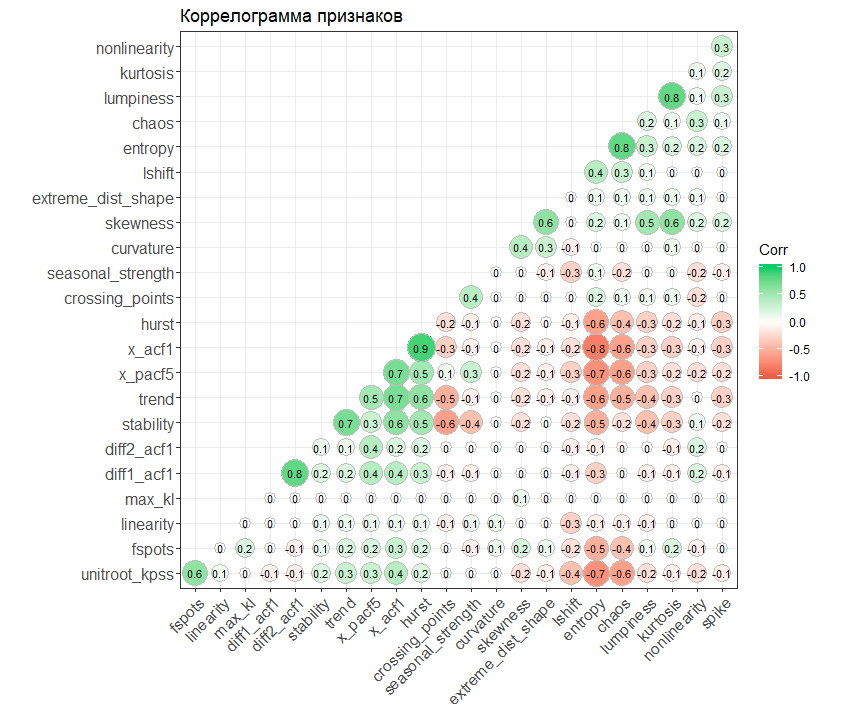
\includegraphics[width=0.9\textwidth]{corr}%{./Pictures/mainscreen1.png}
	
	\label{corr}
	\caption{Коррелограмма признаков}
	
\end{center}
\end{figure} 

	\begin{figure}[h!]

				\begin{center}
		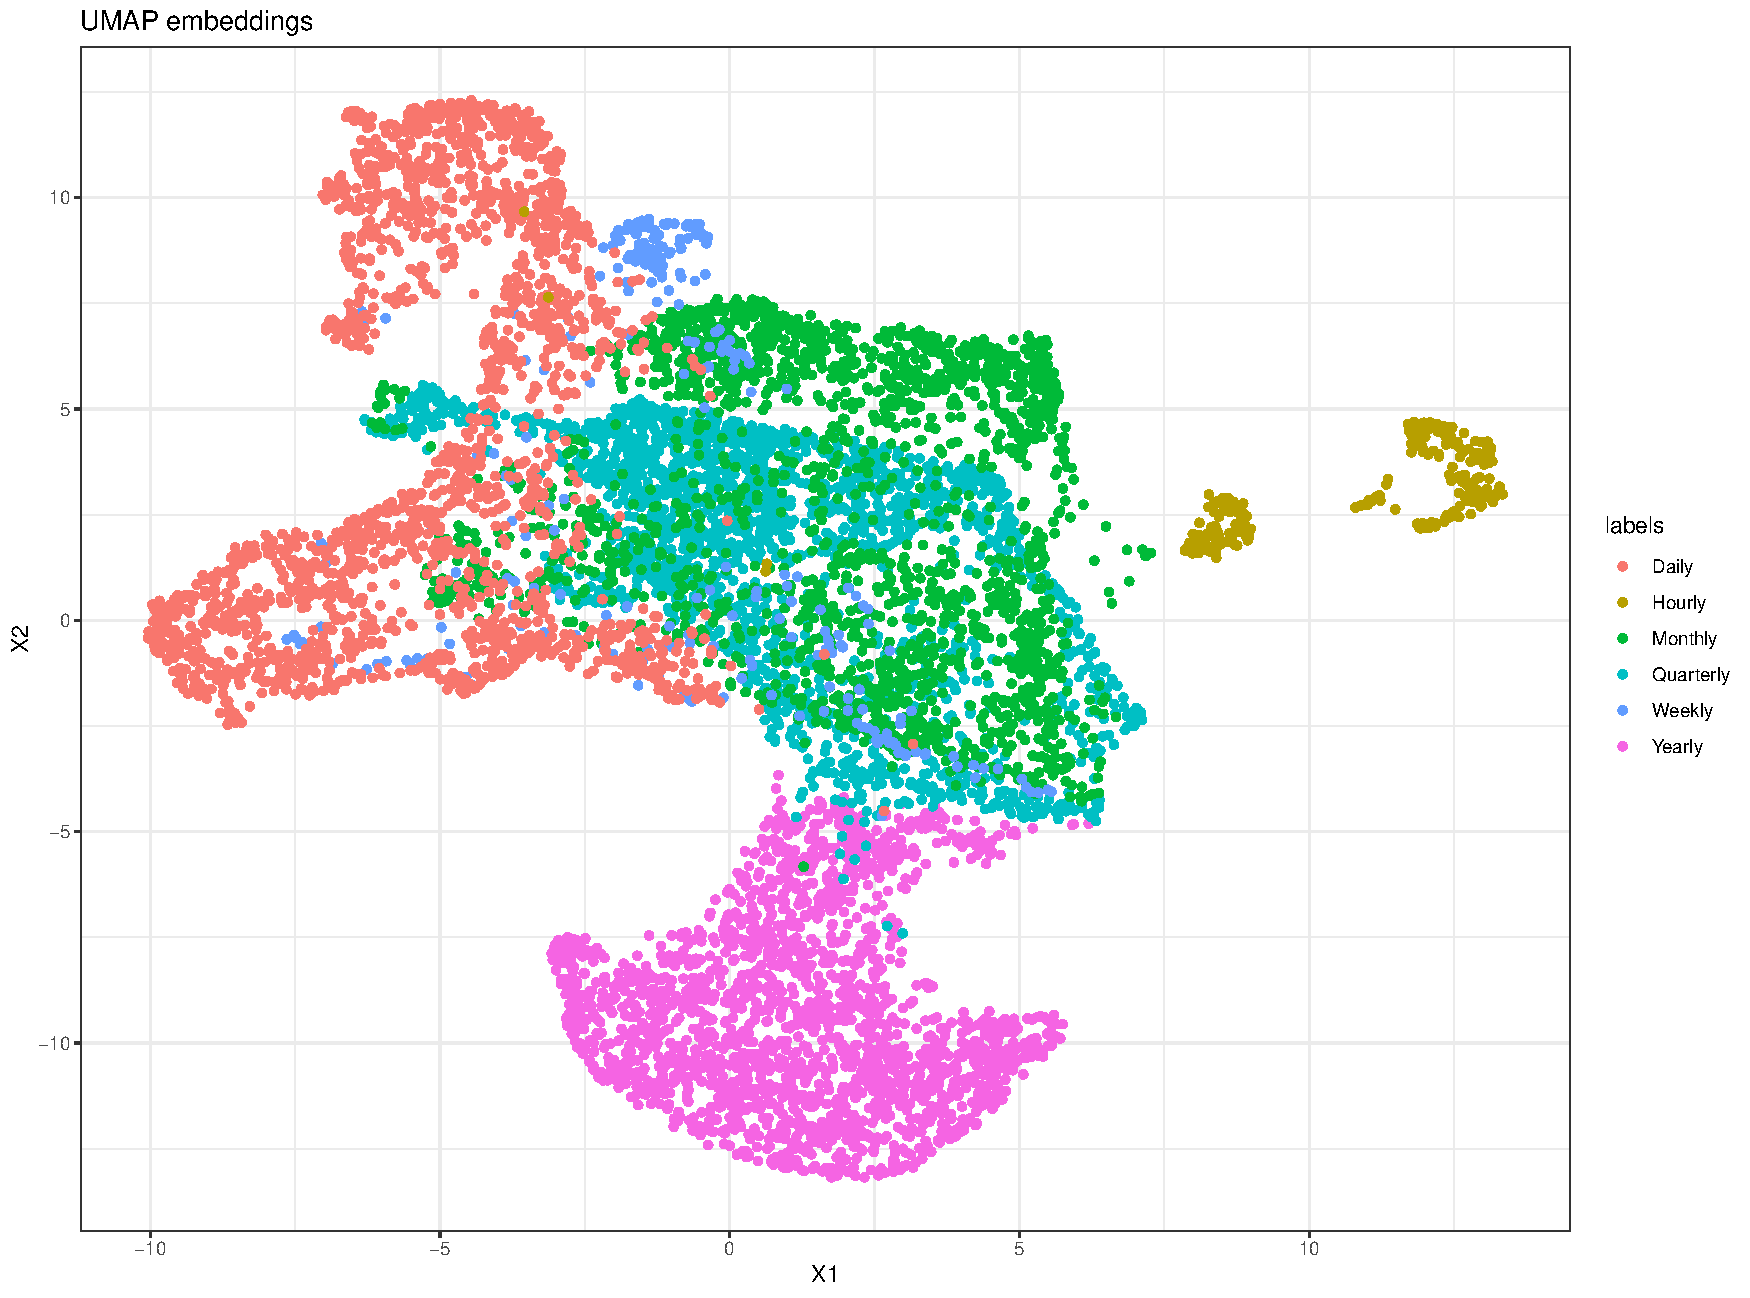
\includegraphics[width=\textwidth]{umap}
		\caption{Эмбеддинги признаков временных рядов в двумерном пространстве}
		\label{umap}
	\end{center}
\end{figure} 


	
	
	
	Также можно заметить сильную положительную корреляцию показателя Хёрста и автокорреляции первого порядка и сильную отрицательную корреляцию автокорреляции первого порядка и спектральной энтропии. 
	
	Теперь попробуем посмотреть, выделяются ли классы периодичности рядов по своим признакам. Для этого используем нелинейный алгоритм UMAP (Uniform Manifold Approximation and Projection). Он группирует наблюдения в зависимости от близости объектов. Что важно, при анализе результатов нельзя ничего сказать о различиях между объектами, только об их близости. Результаты можно увидеть на Рис. \ref{umap}.
		

	
	Как можно заметить, годовые  и почасовые ряды хорошо отделяются от остальных. Следовательно, они имеют специфические характеристики. Также очевидно, что квартальные, месячные и недельные ряды весьма близки по своим характеристикам. Дневные данные также более-менее выделяются в отдельный кластер, однако также их характеристики могут быть близки к квартальным, месячным или недельным данным.
	

	
	
	Теперь попытаемся выяснить, какие признаки более характерны для каждого типа рядов. Для этого мы используем PCA (Principal Component Analysis).  Этот метод поможет понизить размерность наших данных, определив, какие две линейные комбинации признаков описывают основную часть дисперсии выборки. Иначе говоря, вся выборка будет описана двумя ортогональными векторами вместо двадцати трёх, и при этом будет сохранён максимум информации о данных. Данный подход можно найти в ряде работ:  \cite{visual}, \cite{start}, \cite{pca},\cite{anomalous}
	
		
	

В таблице в Приложении \ref{prcomp} представлены веса первых двух главных компонент, описывающих 41.5\% и 19.3 \% дисперсии исходных данных соответственно. Следовательно, суммарно эти характеристики описывают 60.8\% дисперсии. Данные вектора мы получаем на выходе алгоритма. Взвешивая с этими весами вычисленные признаки каждого ряда (центрированные), мы получим точку в признаковом пространстве двух первых компонент. Таким образом, взвесив признаки всех рядов с помощью этих весов, мы можем получить двумерное представление наших данных. Визуализацию можно увидеть на Рис.~\ref{pca}.

Как мы можем видеть, вновь кластеры дневных и годовых временных рядов резко выделяются, а оставшиеся  группы довольно сильно накладываются друг на друга. К тому же их кластеры не имеют чёткой формы. Тем не менее, все кластеры всё равно довольно хорошо различимы. 

Как уже сказано выше, характеристики временных рядов были отнормированы и теперь распределены на отрезке $ [0, 1] $. Следовательно, мы можем визуализировать силу каждой характеристики на данном рисунке. Примеры таких визуализаций можно увидеть на Рис. \ref{fin_str}. Полный набор визуализаций силы характеристик можно найти в Приложении \ref{strength}.

Внимательно взглянув на рисунки можно заметить несколько интересных особенностей:



\begin{enumerate}
	\item Lumpiness, Kurtosis, Maximum KL-divergence и Spike являются почти константными признаками. Скорее всего это связано с наличием небольшого количества выбросов, которые при нормировке сделали признаки нерепрезентативными.
	
	
	
	\item Более частотные ряды (недельные, дневные) более склонны к нестационарности. Скорее всего это связано с тем, что у более частотных данных чаще происходят структурные сдвиги. 
	
	
	\item Взглянув на графики Unitroot KPSS и энтропии можно заметить, что более склонны к прогнозированию более стационарные ряды, что, в общем, логично. Чем больше потенциальных структурных сдвигов, тем сложнее выстроить прогноз. 
	
	\item Аналогичный с предыдущим вывод можно сделать и о показателе стабильности. У нестационарных рядов дисперсия выборочных средних ожидаемо выше, чем у стационарных.

	\item Ряды с высокой энтропией часто имеют и высокую хаотичность. Этот результат также совместим с логикой. Чем больше в данных хаоса, тем сложнее их прогнозировать и тем более сложная модель необходима.
	
	\item Алогичен результат вычисления характеристик линейности и нелинейности. По сути, они должны быть если и не диаметрально противоположными, то хотя бы проявлять какой-то антагонизм. Однако на характеристиках мы этого не наблюдаем. Это скорее всего связано с разными подходами в методике подсчёта. 
	
	\item Интересны рисунки автокорреляции после первого и второго дифференцирований. Наиболее коррелированные ряды смещаются к полюсам второй главной компоненты. 
\end{enumerate}


\begin{figure}[!h] 
	\begin{center}
		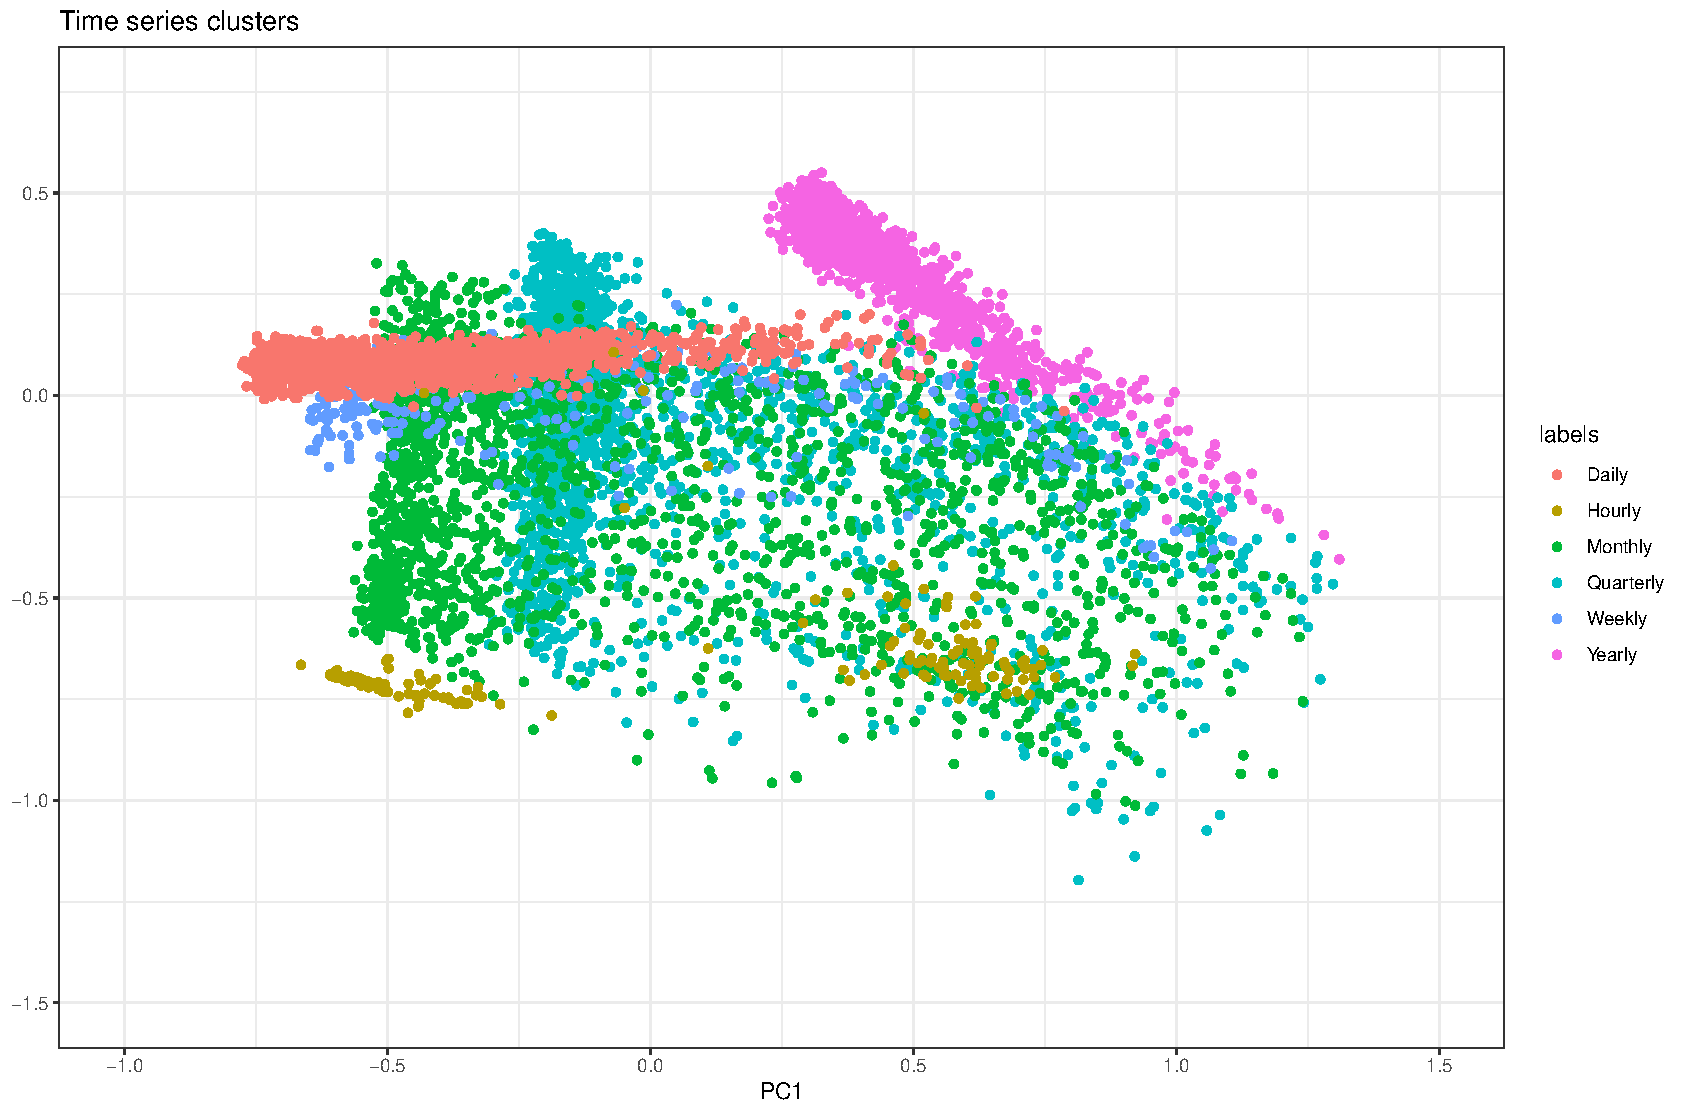
\includegraphics[width=0.9\textwidth]{pca}%{./Pictures/mainscreen1.png}
		\caption{Выборка в пространстве первых главных компонент}
		\label{pca}
	\end{center}

\end{figure} 
	
	\begin{figure}[!h]
	\begin{center}
		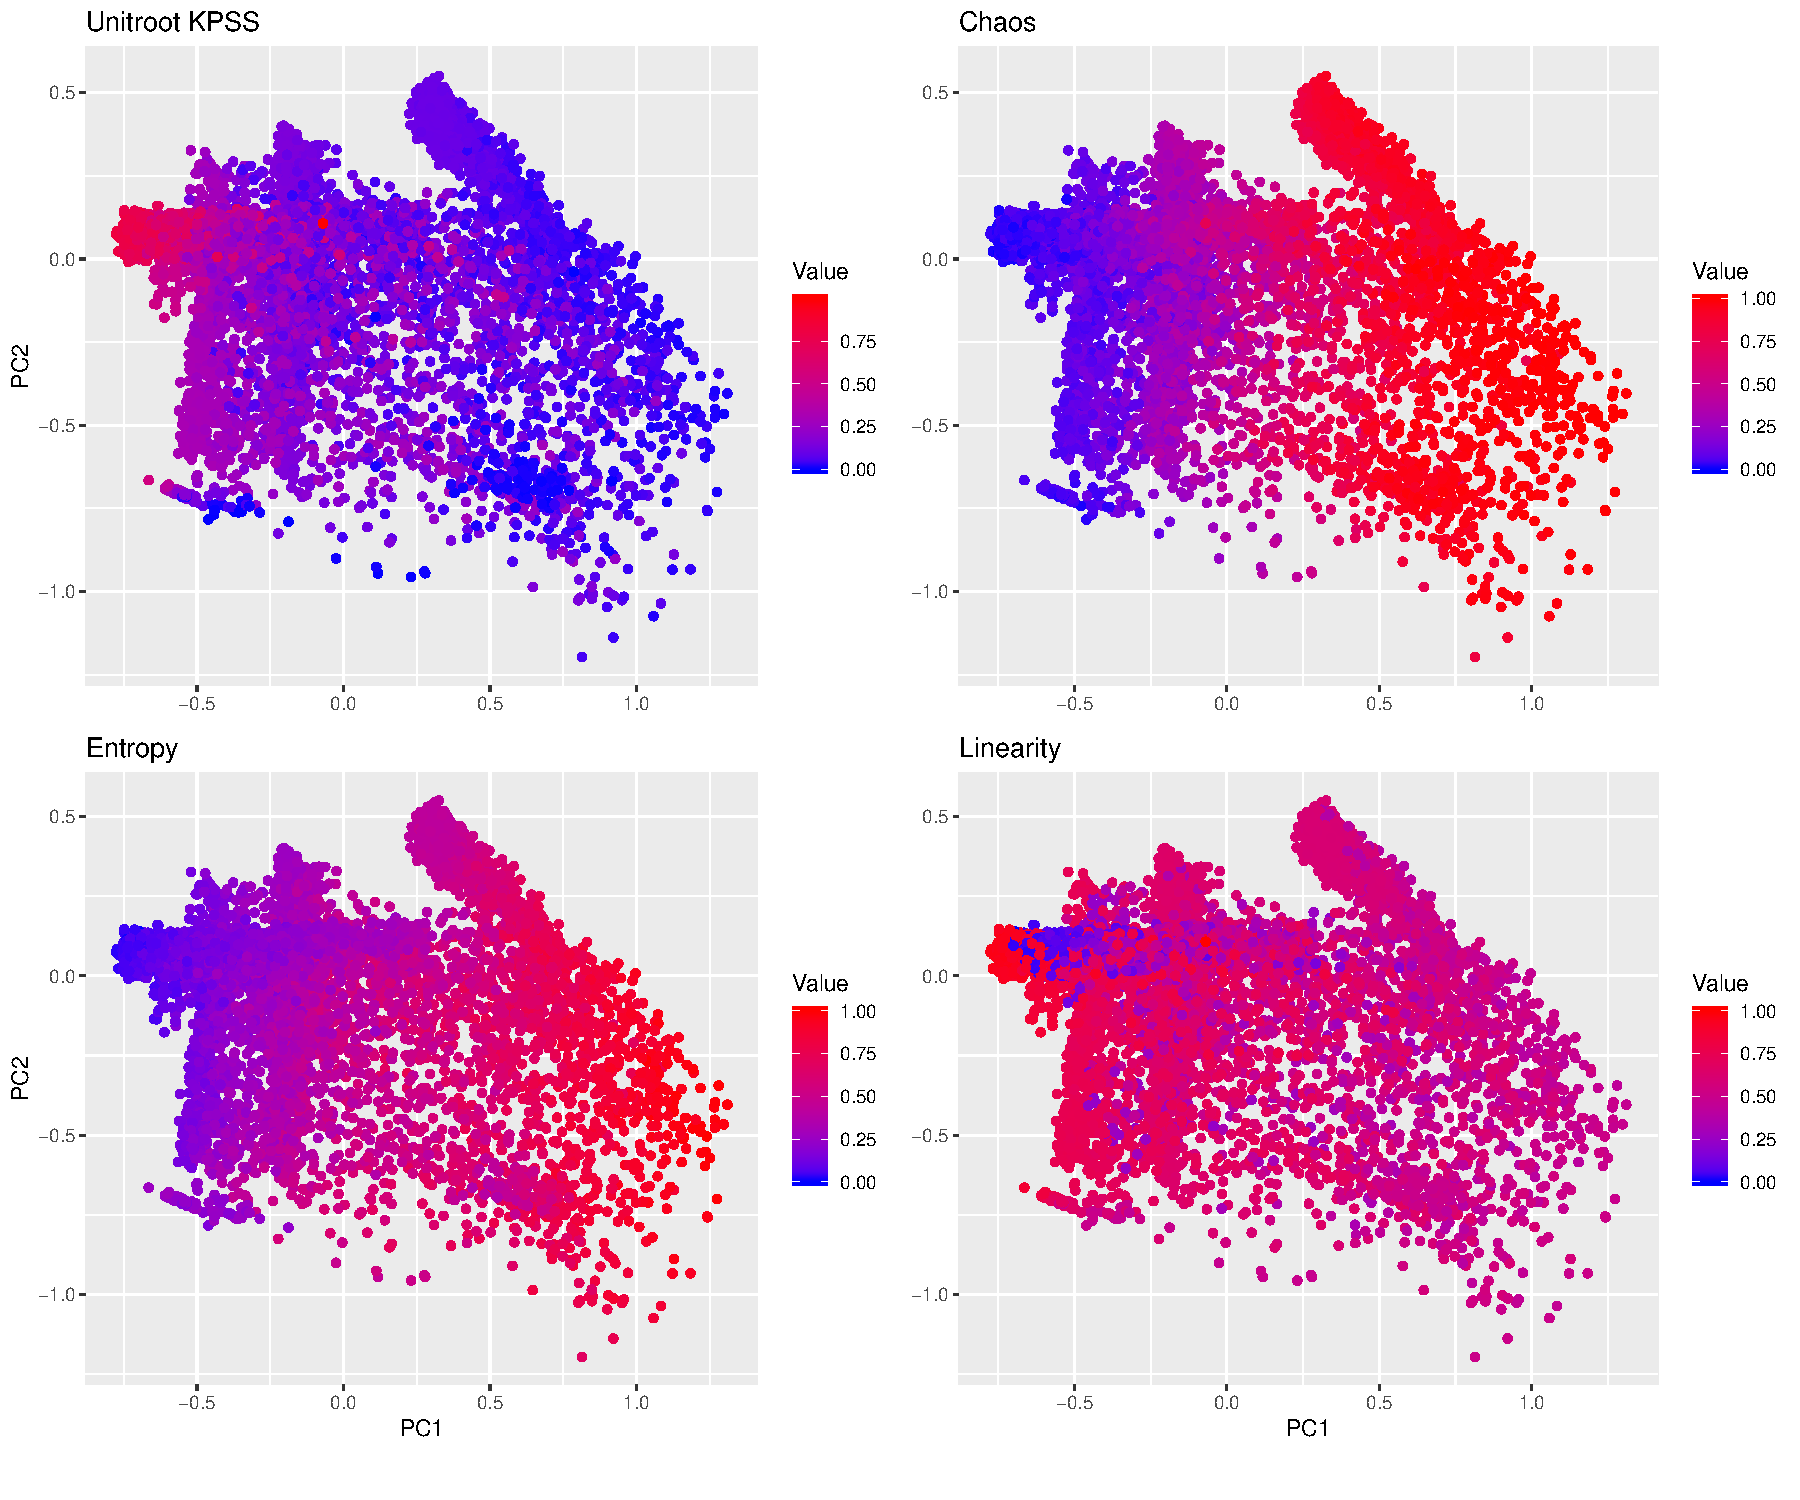
\includegraphics[width=0.8
		\textwidth]{fin_str}%{./Pictures/mainscreen1.png}
		\caption{Сила характеристик в выборке}
		\label{fin_str}
	\end{center}
\end{figure} 

\newpage
\section{Генерация дополнительных рядов в выборке}

Как легко заметить, признаковом пространстве первых двух главных компонент присутствуют белые пятна или просто области, в которых ряды сосредоточены более разреженно. Для того чтобы несколько исправить это положение ниже будет описан способ генерации временных рядов на основе их ближайших соседей в признаковом пространстве. Так можно будет получить новые временные ряды с необходимыми характеристиками! Этот подход используется, например, в \cite[стр.18]{start} и \cite[стр.10]{visual}.

Для этого мы воспользуемся специальным пакетом R под названием GA. Он использует базовые принципы биологической эволюции и селекции для решения оптимизационных задач. Основная идея базируется на том, что наиболее совершенные индивиды доминируют над более слабыми. В процессе смены поколений индивидов с некоторыми ограничительными условиями будут происходить такие процессы как селекция, кроссовер и мутация. 

Теперь перейдём непосредственно к реализации. Генерировать новые ряды будем отдельно по каждому кластеру периодичности. Визуализации для примера будут показаны на годовых рядах.

Первым шагом необходимо определить целевые точки генерации новых рядов. Для этого необходимо сгенерировать сетку всех возможных целей. Будем считать, что характеристики целей за пределом выпуклого полигона недостижимы в данном классе. Следовательно, сгенерируем сетку только внутри полигона. Для этого удобно воспользоваться соответствующими функциями R:
\begin{enumerate}
	\item chull() (пакет "grDevices"\ ) - выделяет на основе набора точек вершины выпуклого полигона.
	\item points.in.polygon() (пакет "sp"\ ) - проверяет, какие точки из заданного набора находятся внутри указанного полигона.
\end{enumerate}	

Результат этого подготовительного этапа можно видеть ниже на первом графике Рис.~ \ref{gen}.

Вторым этапом является фильтрация попавших внутрь полигона точек. Мы хотим избежать репликации исходных данных. Cледовательно, нужно оставить только незаполненные области. На втором графике Рис. \ref{gen} можно увидеть результат фильтрации данных. На данном графике остались только точки, расстояние от которых до их ближайшего соседа не меньше $ 0.02 $. Данный параметр является произвольным и зависит только необходимого количества финальных целевых точек.

Все целевые точки обсчитать в данной работе не представляется возможным за неимением такого количества вычислительного времени, поэтому из целевого множества случайно выбираются $ 300 $ точек (для недельных и часовых данных по $ 100 $ точек), которые и являются итоговыми целевыми точками.
\begin{figure}[!h]
	
	\begin{center}
		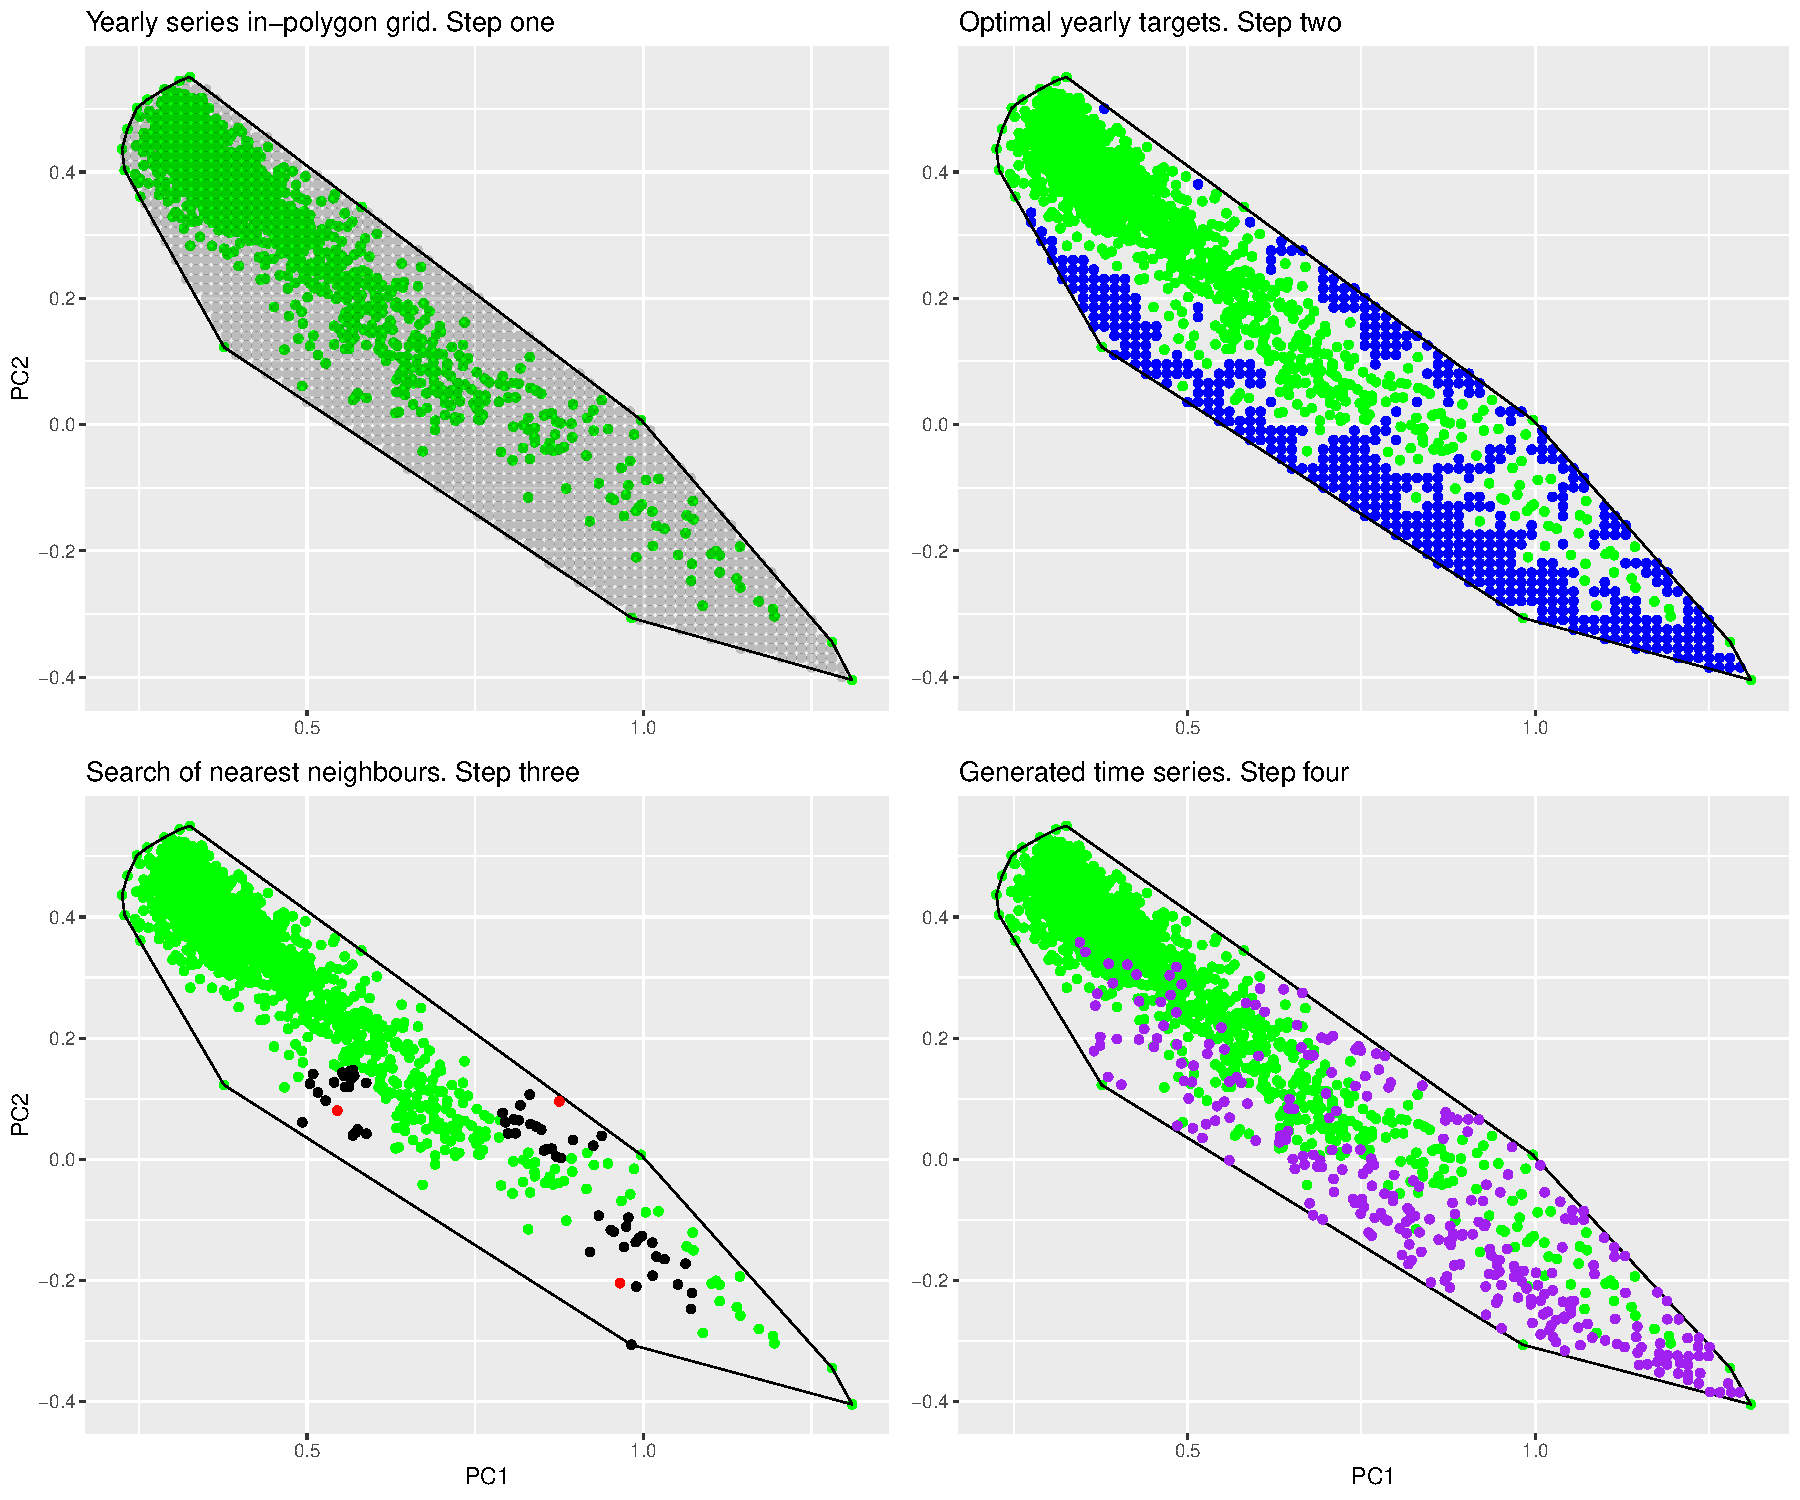
\includegraphics[width=
		\textwidth]{generation_grid}%{./Pictures/mainscreen1.png}
		\caption{Этапы генерации  рядов}
		\label{gen}
	\end{center}
\end{figure} 

На третьем шаге необходимо определить, какая стартовая популяция будет принадлежать каждой целевой точке. В этом плане тоже будем избегать изысков, а просто возьмём десять ближайших соседей в признаковом пространстве. Это улучшит сходимость алгоритма. Можно взять и больше соседей, но тогда на длинных рядах придётся серьёзно пожертвовать скоростью вычислений. Тем не менее, процесс можно распараллелить и, при наличии достаточных мощностей, получить результат в разумные сроки. Визуализацию третьего шага можно увидеть на третьем графике Рис. \ref{gen}.

Четвёртый шаг является непосредственно генерацией рядов и является самым сложным.	Опишем пошагово, что происходит на этом этапе для одного каждого временного ряда. Обозначим текущую целевую точку за $ T_i, i = 1, 2, ..., N_t $

Для начала формируется стартовая популяция. Как уже упоминалось, стартовой популяцией мы будем считать десять ближайших соседей в признаковом пространстве первых двух главных компонент. Далее на каждой итерации с этой популяцией происходят преобразования, обусловленные генетическими алгоритмами. Лучшим в данной популяции признаётся ряд, наиболее близкий к целевой точке.

Следующим моментом, который следует пояснить, является процесс оптимизации. Он происходит по следующей схеме: 
	
	\begin{enumerate}
		\item Для каждого кандидата $ j \in \{1, 2, ..., N_p\} $ в текущей популяции вычисляется вектор характеристик, который проецирутся на двумерное пространство первых двух главных компонент. Проецирование выполняется с помощью вычисленных ранее весов (см. Приложение \ref{prcomp}). Обозначим эту двумерную проекцию как $ PC_j $.
		
		\item Вычисляется близость каждого кандидата к целевой точке
		
		\[ Fitness(j) = -\sqrt{(|PC_j - T_i|^2)} \]
		
		\item С помощью кроссовера, мутаций и выживания сильнейших кандидатов формируется следующее поколение с целью повышения средней близости к целевой точке каждого следующего поколения. 
	\end{enumerate}

Эта процедура задаёт итеративный процесс подбора наилучших кандидатов для каждой целевой точки. Также на процесс оптимизации были наложены несколько ограничений и терминальных условий:

\begin{enumerate}[\Sun]
	\item Вероятность кроссовера была равна $ 0.8 $, а вероятность мутации -- $ 0.2 $
	\item Терминальное количество поколений: $ 500 $
	
	\item Терминальное значение максимизируемой функции: $ -0.001 $
	
	\item Терминальное количество поколений без улучшения максимизируемой функции: $ 100 $
\end{enumerate}

Процесс оптимизации можно легко проиллюстрировать. На Рис. \ref{optim} можно увидеть зависимость среднего значения оптимизируемой функции по всем индивидам от поколения для случайно выбранного ряда. 
\begin{figure}[!h]
	\begin{center}
		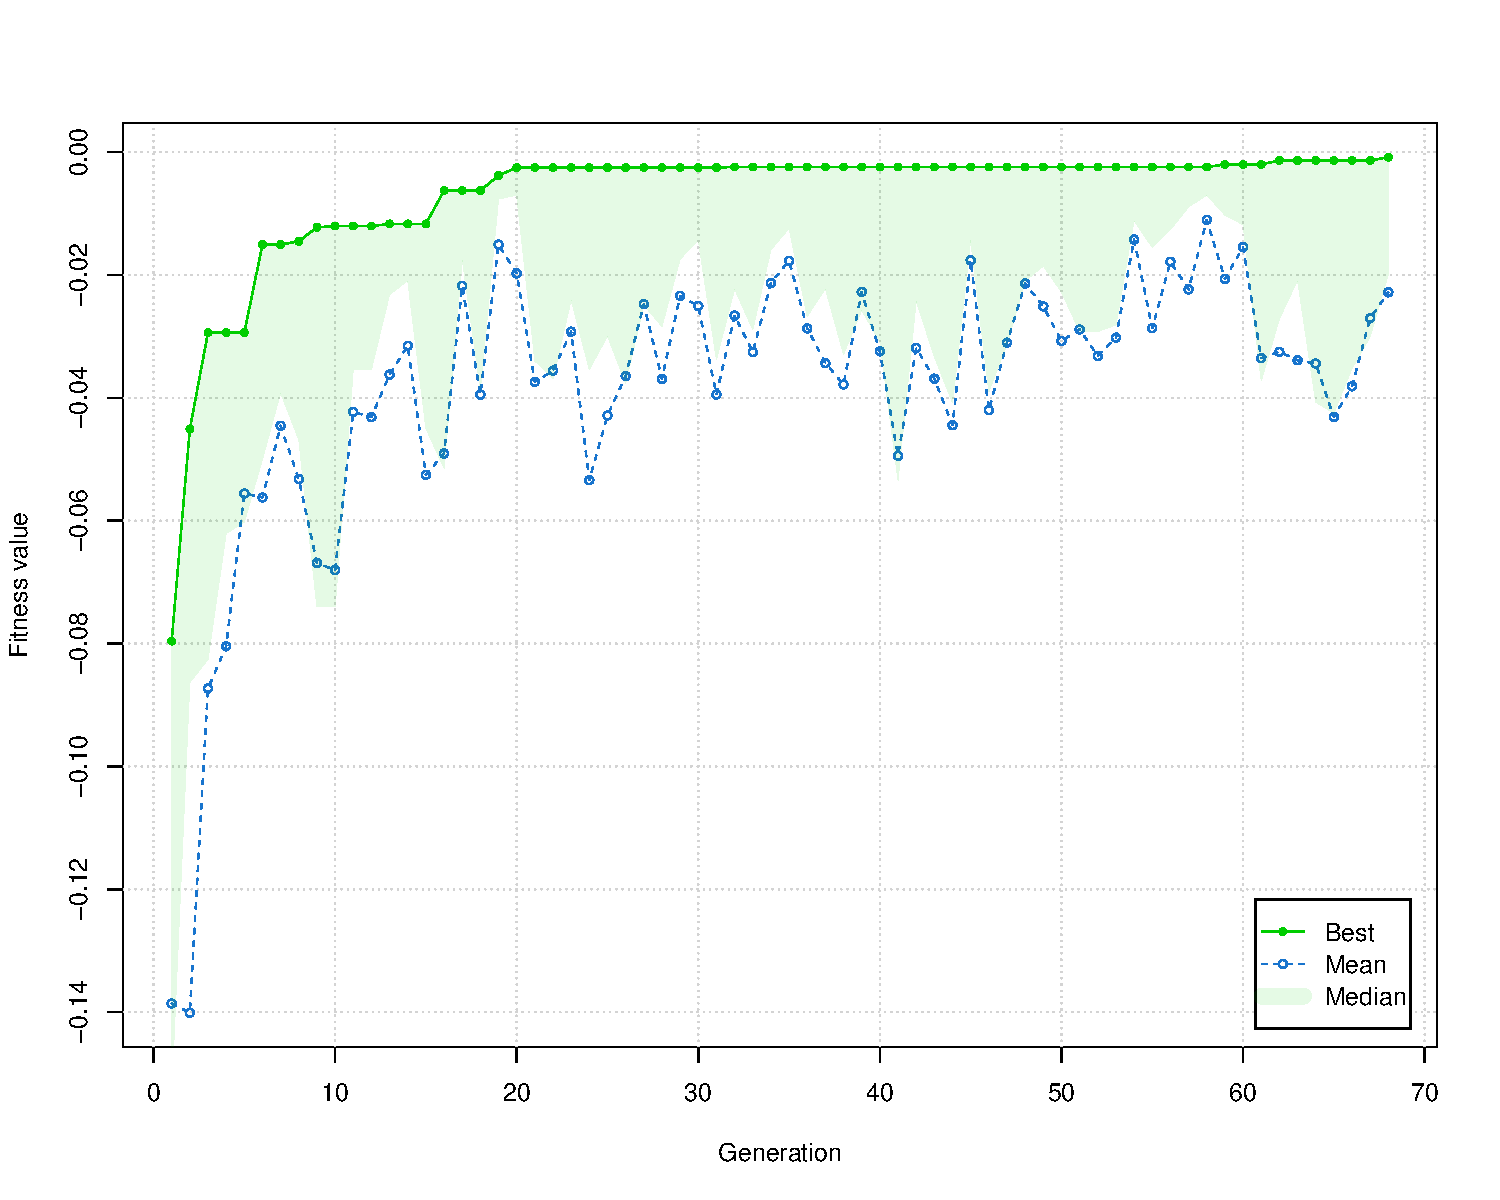
\includegraphics[width=0.8
		\textwidth]{optim}%{./Pictures/mainscreen1.png}
		\caption{Процесс оптимизации}
		\label{optim}
	\end{center}
\end{figure} 

Также на графике видно значение функции для наилучшего кандидата. Как видим, в данном случае это значение превысило терминальное, и на семидесятом поколении цель была достигнута. 


Подобным образом для каждого кластера, кроме почасовых рядов, было сгенерировано определённое количество рядов. Для групп по $ 2000 $ рядов генерировались дополнительно $ 300 $ рядов, а для малочисленных недельных рядов -- $ 100 $.

 Однако, не все временные ряды идеально подогнались под целевые точки. Это можно заметить по четвёртому графику на Рис. \ref{gen}. Можно заметить, что некоторые сгенерированные ряды попали в область, в которой целевых точек не было в принципе. Ничего критичного в этом нет. Также некоторые финальные кандидаты и вовсе не попали внутрь полигона. Это уже считается недопустимым, и они были отфильтрованы как нерелевантные. Итоговые результаты после генерации можно увидеть в таблице на Рис. \ref{targets}.
 
 \begin{wrapfigure}{r}{0.5\textwidth} 
 	\begin{center}
 \begin{tabular}{|
 		>{\columncolor[HTML]{91FF91}}l |l|l|}
 	\hline
 	\textbf{Класс} & \cellcolor[HTML]{91FF91}\textbf{\begin{tabular}[c]{@{}l@{}}Исходное\\ количество\end{tabular}} & \cellcolor[HTML]{91FF91}\textbf{\begin{tabular}[c]{@{}l@{}}Итоговое\\ количество\end{tabular}} \\ \hline
 	\textbf{Yearly} & 300 & 285 \\ \hline
 	\textbf{Quarterly} & 300 & 297 \\ \hline
 	\textbf{Monthly} & 300 & 297 \\ \hline
 	\textbf{Weekly} & 100 & 100 \\ \hline
 	\textbf{Daily} & 300 & 294 \\ \hline
 	\textbf{Hourly} & -- & -- \\ \hline
 	\textbf{Total} & 1300 & 1273 \\ \hline
 \end{tabular}
 		\caption{Задачи и итоги генерации рядов}
 		\label{targets}
 		
 		
 	\end{center}
	
 \end{wrapfigure} 
 
 
 
 Тем не менее, глядя на график сгенерированных рядов, можно сказать, что цель достигнута. Наименее плотные области кластера заполнены соответствующими по характеристикам временными рядами. 
 Визуализацию результатов генерации можно увидеть в Приложении \ref{all_gen}.
 
 Касательно вопроса о том, почему не генерировались почасовые временные ряды и почему они вовсе не будут далее использоваться в вычислениях. Дело в том, что форма кластера временных рядов из-за наличия в них пары выбросов и двух разрозненных групп (см. Рис. \ref{pca}), генерировать внутри кластера сетку становится бессмысленным. Слишком низка плотность рядов в основном пространстве кластера. Дополнительным фактором служит длина рядов. Так как они существенно длиннее чем в других кластерах, серьёзно возрастает требуемое время вычислений. Забегая вперёд, время подбора модели функцией $ auto.arima() $, встроенной в R, превысило $ 20 $ минут. В связи с невозможностью в данном случае параллельных вычислений, почасовые ряды на данном этапе исключаются из обзора. 
 
 Прозорливый читатель заметит, что в таком случае хорошо бы воспроизвести заново все вычисления, начиная от PCA, но в данной работе автор признаёт техническую невозможность сделать это и кается в своих грехах и самонадеянности. 
 
	 В завершение данной главы предлается взглянуть на пример симулированного ряда. На Рис. \ref{ex_gen} можно увидеть случайно выбранный сгенерированный месячный ряд и двух его ближайших соседей.
 
 \begin{figure}[!h]
 	
 	\begin{center}
 		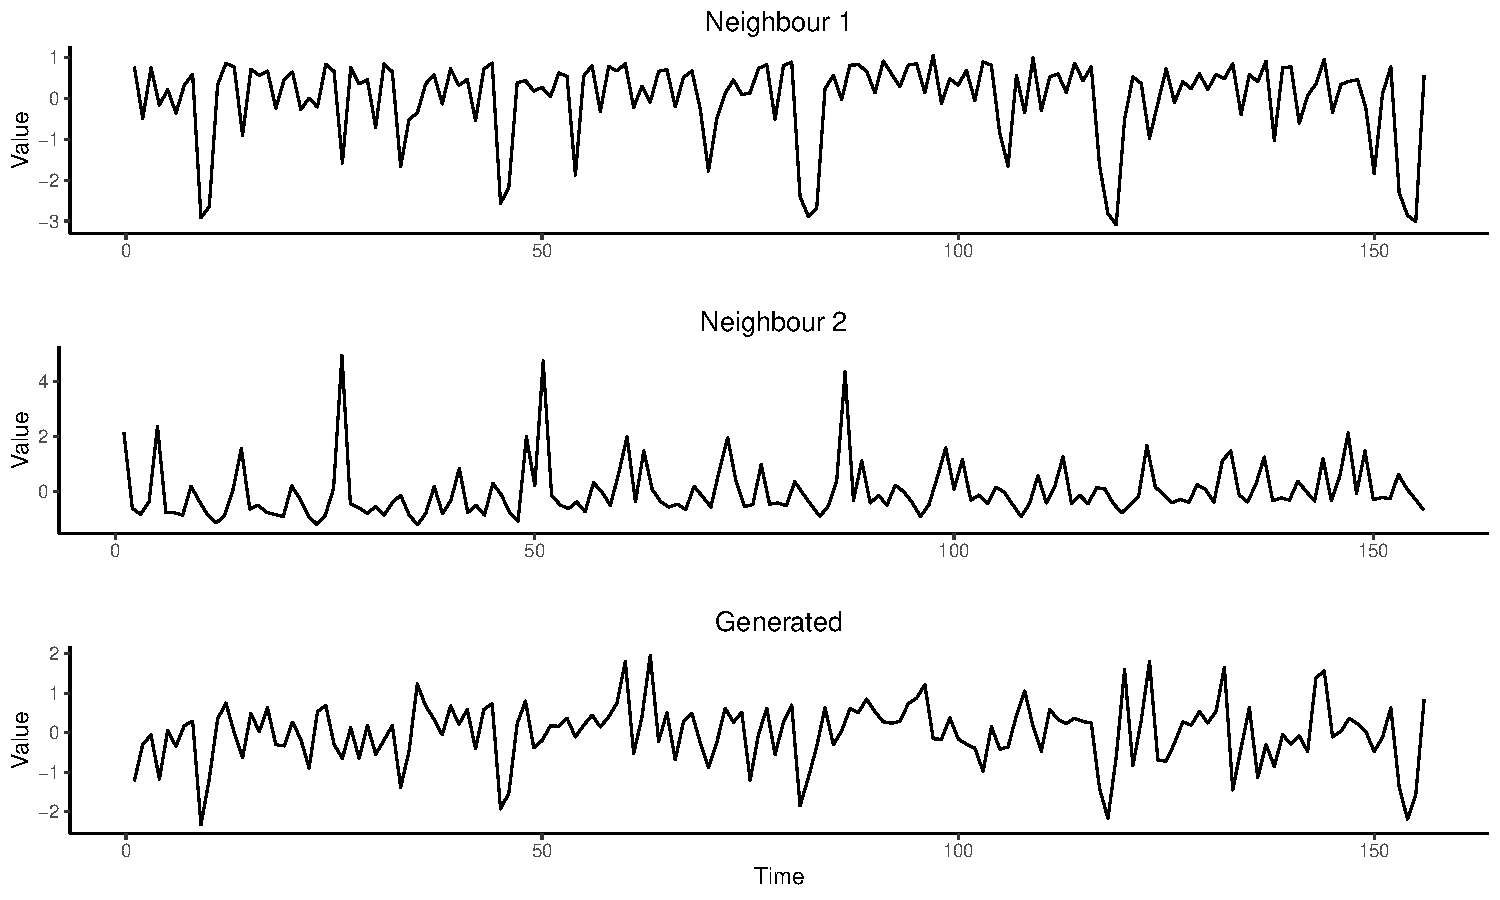
\includegraphics[width=
 		0.9\textwidth]{gen_and_neighbours}%{./Pictures/mainscreen1.png}
 		\caption{Пример сгенерированного ряда}
 		\label{ex_gen}
 	\end{center}
 \end{figure} 
 
\newpage
 \section{Модели прогнозирования временных рядов}
 
 В данном разделе будут описаны модели прогнозирования  временных рядов, которые позже будут использованы для разметки мета-данных. В данной работе будет использован набор из девяти одномерных моделей прогнозирования. 
 
 \begin{enumerate}
	 \item Наивный прогноз.
	 
	  В качестве прогноза берётся последнее известное значение тренировочной части ряда. Таким образом, получается "плоский"\ прогноз. Данная модель будет использоваться в качестве бенчмарка для остальных.
	 
	 \item Сезонный наивный прогноз.
	 
	 Прогнозом служит значение, временного ряда, имевшее место $ k $ шагов назад относительно прогнозируемого значения, где $ k $ -- период сезонности. Для годовых данных этот метод эквивалентен наивному прогнозу.
	 
	 \item Случайное блуждание с дрейфом.
	 
	 Данная модель описывается следующим уравнением:
	 \[ Y_t = \alpha + Y_{t-1} + \epsilon_t \]
	 
	 Значение временного ряда в момент $ t $ описывается как сумма значения на предыдущем шаге, константы $ \alpha $ (дрейф) и белого шума $ \epsilon_t $ c нулевым математическим ожиданием и дисперсией $ \sigma^2 $. Процесс случайного блуждания с дрейфом не является "mean-reverting"\ , то есть не возвращается к долгосрочному среднему на бесконечном временном горизонте, а устремляется от него. Дисперсия прогноза этого процесса положительно зависит от времени и устремляется в бесконечность при росте горизонта прогнозирования. 	
	 
	 Прогноз данной модели вычисляется по формуле:
	 
	 \[ \hat{Y}_{T+h| T} = E(Y_{T+h} | I_T) = \alpha + Y_T, \quad \text{ где } I_T - \text{ информация, доступная к периоду T}\]
	 Эта модель просто и быстро оценивается, а также широко используется для прогнозирования нестационарных рядов, таких как, например, цены акций.  
	 
	 \item Простое экспоненциальное сглаживание.
	 
	 Идея данной модели весьма проста. Наивный прогноз слишком сильно полагается на последнее значение. Хотелось бы включить в модель опору на предыдущие значения. Самым простым решением в данном случае кажется простое усреднение:
	 
	 \[   \hat{Y}_{T+h| T} = \frac{1}{t}\sum_{t = 1}^{t}Y_t\]
	 
	 Однако эту модель можно модифицировать, присвоив последним значениям большие веса, а отдалённым - меньшие. Так появилась модель простого экспоненциального сглаживания, формулу прогноза которой можно записать следующим образом: 
	 
	 \[   \hat{Y}_{T+1| T} = \alpha Y_T	 + \alpha(1 - \alpha)Y_{T-1} + \alpha(1 - \alpha)^2Y_{T - 2} + \cdots,\]
	 
	 где $ \alpha \in [0, 1]$ является параметром сглаживания. Чем $ \alpha $ больше, тем больший вес придаётся последнему наблюдению. 
	 
	 \item ETS - модель.
	 
	 Данный метод предлагает автоматический процесс подбора ETS-модели для временного ряда на основе классификации, описанной в \cite{ets}. Алгоритм полностью автоматизирован и требует на вход только непосредственно временной ряд. Этот метод хорошо подходит для трендированных и сезонных данных, так как модель предполагает широкий список возможных вариантов моделирования компонент (тренд, сезонность и ошибка). 
	 
	 \item Theta - модель
	 
	 Тета-модель была представлена в \cite{theta}. Эта модель отлично зарекомендовала себя в соревновании M3. В общем виде она является частным случаем ETS(A,A,N) - модели. Поясним это, используя стандартную спецификацию данной модели:
	 
	 \[ 
	 \begin{cases}
	 	y_t = l_{t-1} + b_{t - 1} + \epsilon_t\\ 
	 	l_t = l_{t - 1} + b_{t - 1} + \alpha \epsilon_t\\
	 	b_t = b_{t - 1} + \beta \epsilon_t
	 \end{cases} 
	  \]
	  
	  где $ \epsilon_t \sim N(\mu, \sigma^2) $. В общем случае необходимо оценить шесть параметров: $ \alpha, \beta, \sigma^2, l_0, b_0 $. Тета-модель предлагает просто положить $ \beta = 0, l_0 = y_0 $
	 
	 \item ARIMA - модель.
	 
	 Интегрированная модель авторегрессии - скользящего среднего -- это комплексный инструмент для моделирования и прогнозирования временных рядов. Он описывается с помощью устоявшегося обозначения ARIMA(p, d, q)  и состоит из трёх основных частей:
	 
	 \begin{enumerate}[\Sun]
	 	\item $ AR(p) $ обозначает авторегрессионную часть модели порядка $ p $. Под авторегрессией понимается регрессия, где зависимая переменная зависит от $ p $ своих лагов:
	 	
	 	\[   y_t = \beta_0 + \beta_1 y_{t - 1} + \dots + \beta_p y_{t - p}  \]
	 	
	 	\item $ I(d) $ обозначает порядок дифференцирования, или, иным языком, количество взятых разностей. Дифференцирование -- это способ ухода от нестационарности временного ряда путём перехода от исходных наблюдений к их изменениям. Говоря языком формул, первая разность будет иметь вид $ y'_t = y_t - y_{t - 1} $
	 	
	 	\item $ MA(q) $ обозначает, что в модель добавляется элемент скользящего среднего порядка $ q $. Она может быть описана регрессионным уравнением, где в качестве независимых переменных служат ошибки $ \epsilon_t $:
	 	
	 	\[ y_t = \beta_0 + \epsilon_t - \theta_1 \epsilon_{t - 1}  + \dots + \theta_{q} \epsilon_{t - q}\]
	 \end{enumerate}
 
 Определение параметров порядка модели ($ p, d, q $) является непростой задачей. Существует эффективный алгоритм поиска оптимальных параметров, который и реализован в функции $ auto.arima() $ пакета $ forecast $ для R. Он подбирает лучшую модель на основе информационных критериев (AIC, AICc, BIC). \cite{arima}  Однако следует заметить, как уже упоминалось выше, данный метод серьёзно деградирует относительно времени вычислений на длинных рядах.
 
 \item TBATS (Trigonometric, Box-Cox transformation, ARMA, Trend, Seasonality)
 
 Данная модель является одной из модификаций модели Хольта-Винтерса (ETS(A,A,A)). Одним из достоинств модели является моделирование постепенно изменяющейся сезонности. Однако недостатком может являть низкая скорость оценки, особенно на длинных рядах.
 
 Разберём модель подробнее. Её первой отличительной особенностью является автоматическое применение применение трансформации Бокса-Кокса:
 
 \begin{equation*}
 	y_t^\lambda = 
 	\begin{cases}
 	\frac{y_t^\lambda - 1}{\lambda}, \lambda \neq 0\\
 	\ln(y_t), \lambda = 0
 	\end{cases}
 \end{equation*}
 
 Наблюдения моделируются следующим образом:
 
 \begin{equation}
 	y_t^\lambda = l_{t - 1} + \phi b_{t - 1} + \sum_{i = 1}^{M} s_{t - m_i}^{(i)} + d_t,
 	\label{four}
 \end{equation}	
 
 где 
 
 \[ b_t = (1 - \phi)b + \phi b_{t-1} + \beta d_t \text{ отражает глобальный тренд}\]
 \[l_t = l_{t - 1} + \phi b_{t - 1} + \alpha d_t \text{ отражает локальный тренд} \]
 
 \[d_t = \sum_{i = 1}^{p}\phi_i d_{t - i} + \sum_{j = 1}^{q} \theta_j \epsilon_{t - j} + \epsilon_t \text{ отражает ошибки в форме ARMA} \]
 
 В уравнении \ref{four} имеется $ M $ сезонных периодов, каждый из которых в свою очередь состоит из $ s_t^{(i)} = \sum_{j = 1}^{k_i}s_{j, t}^{(i)}$. Каждое из слагаемых моделируется при помощи ряда Фурье:
 
 \[ s_{j, t}^{(i)} = s_{j, t - 1}^{(i)}cos\lambda_j^{(i)} + s_{j, t - 1}^{*(i)} sin\lambda_j^{(i)} + \Gamma_1^{(i)} d_t\]
 
  \[ s_{j, t}^{(i)} = - s_{j, t - 1}^{(i)}sin\lambda_j^{(i)} + s_{j, t - 1}^{*(i)} cos\lambda_j^{(i)} + \Gamma_2^{(i)} d_t\]
 
 \item Нейронная сеть
 
 Последней моделью в нашем списке будет нейронная сеть прямого распространения с одним скрытым слоем. Размерность скрытого и входного слоёв будут определяться автоматически на основе информационного критерия AIC.  Эта модель быстро оценивается за счёт своей простоты. Различные модификации данной модели широко используются в прогнозировании. Полноценное исследование можно найти в \cite{nnet}. 
 
\end{enumerate}

\newpage

\section{Разметка данных}

Теперь необходимо разметить данные, которые далее будут поданы на вход мета-алгоритму. Для этого необходимо на каждом ряду обучить по девять моделей и выделить модель с наименьшей ошибкой. 



\begin{wrapfigure}{r}{0.4\textwidth} 
\begin{tabular}{|
		>{\columncolor[HTML]{91FF91}}l |l|l|}
	\hline
	\textbf{Класс\textbackslash{}Длина} & \cellcolor[HTML]{91FF91}\textbf{Train} & \cellcolor[HTML]{91FF91}\textbf{Test} \\ \hline
	{\color[HTML]{000000} \textbf{Yearly}} & 27 & 3 \\ \hline
	{\color[HTML]{000000} \textbf{Quarterly}} & 54 & 6 \\ \hline
	{\color[HTML]{000000} \textbf{Monthly}} & 140 & 16 \\ \hline
	{\color[HTML]{000000} \textbf{Weekly}} & 283 & 32 \\ \hline
	{\color[HTML]{000000} \textbf{Daily}} & 450 & 50 \\ \hline
\end{tabular}
\caption{Горизонты прогнозирования}
\label{len}
\end{wrapfigure}

Но прежде чем прогнозировать, нужно определиться, насколько далеко. То есть, необходимо разбить каждый ряд на тренировочную часть и тестовую. Одинаковый горизонт прогнозирования несколько алогичен из-за различной длины рядов, поэтому было выбрано разделение на основе длины ряда.

 $ 90\% $ длины служило тренировочной частью, а оставшиеся $ 10\% $ - тестовой. Соответственно, на тренировочной части вычислялись характеристики временного ряда и обучались модели прогнозирования, а на тестовой вычислялись ошибки прогнозов моделей. Горизонты прогнозирования можно увидеть в таблице на Рис. \ref{len}.
 
Для оценки качества прогноза была использована симметричная средняя абсолютная процентная ошибка (SMAPE) \cite[стр.13]{smape} :

\[ SMAPE =  \frac{1}{n}\sum_{t = 1}^{n} \frac{|y_t - \hat{y}_t|}{(y_t + \hat{y}_t) / 2} \star 100, \]

где $ n $ обозначает горизонт прогнозирования.
 
 Таким образом были вычислены ошибки всех моделей на всех рядах (исходных и сгенерированных искусственно). Визуализируем ошибки каждой модели. В Приложении \ref{smape} можно увидеть анимацию, визуализирующую ошибки каждого алгоритма на всей выборке. Для просмотра анимации необходимо открыть данную работу в Adobe Reader.
 
 
  Определив для каждого ряда наилучшую модель на основе наименьшей ошибки, разметим наши временные ряды и получим датасет с двадцатью тремя численными характеристиками и факторной зависимой переменной. В следующей главе этот датасет будет использоваться для обучения мета-алгоритма. Также можно визуализировать наименьшую ошибку для каждого наблюдения в выборке. Результат представлен в Приложении \ref{min_smape}. Полученные результаты согласуются с нашими ранними наблюдениями. Максимальную ошибку имеют ряды, имеющие высокую энтропию и уровень хаоса. То есть, эти ряды можно признать плохо прогнозируемыми, что подтвердилось эмпирически.
 
 Из результатов разметки можно извлечь ещё несколько интересных результатов. Для этого взглянем на таблицу на Рис. \ref{counts}.


 
\begin{figure}[!h]
 	\begin{center}
 
\begin{tabular}{|
		>{\columncolor[HTML]{91FF91}}l |
		>{\columncolor[HTML]{FFFFFF}}l |
		>{\columncolor[HTML]{FFFFFF}}l |
		>{\columncolor[HTML]{FFFFFF}}l |
		>{\columncolor[HTML]{FFFFFF}}l |
		>{\columncolor[HTML]{FFFFFF}}l |}
	\hline
	\textbf{Модель\textbackslash{}Класс} & \cellcolor[HTML]{91FF91}\textbf{Yearly} & \cellcolor[HTML]{91FF91}\textbf{Quarterly} & \cellcolor[HTML]{91FF91}\textbf{Monthly} & \cellcolor[HTML]{91FF91}\textbf{Weekly} & \cellcolor[HTML]{91FF91}\textbf{Daily} \\ \hline
	\textbf{Naive} & 204 | 9\% & 161 | 7\% & 112 | 5\% & 39 | 10\% & 90   | 4\% \\ \hline
	\textbf{Seasonal Naive} & -- & 232 |10\% & 266 | 12\% & 39 | 10\% & 230 | 10\% \\ \hline
	\textbf{RW with drift} & 333 | 14\% & 339 | 15\% & 271 | 12\% & 75 | 19\% & 595 | 26\% \\ \hline
	\textbf{SES} & 112 | 5\% & 89   | 3\% & 86   | 4\% & 19 | 5\% & 88   | 4\% \\ \hline
	\textbf{ETS} & 311 | 14\% & 288 | 13\% & 328 | 14\% & 24 | 6\% & 56   | 2\% \\ \hline
	\textbf{ARIMA} & 366 | 16\% & \cellcolor[HTML]{91FF91}443 | 19\% & \cellcolor[HTML]{91FF91}466 | 20\% & 57 | 15\% & 247 | 12\% \\ \hline
	\textbf{Theta} & 166 | 7\% & 127 | 6\% & 100 | 4\% & 11 | 3\% & 152 | 7\% \\ \hline
	\textbf{TBATS} & \cellcolor[HTML]{91FF91}444 | 19\% & 288 | 13\% & 323 | 14\% & 40 | 10\% & 181 | 8\% \\ \hline
	\textbf{Neural net} & 348 | 15\% & 127 | 6\% & 345 | 15\% & \cellcolor[HTML]{91FF91}82 | 21\% & \cellcolor[HTML]{91FF91}655 | 29\% \\ \hline
	\textbf{Total} & 2284 & 2297 & 2297 & 386 & 2294 \\ \hline
\end{tabular}
	\caption{Наиболее успешные модели по каждом классу}
	\label{counts}
\end{center}

\end{figure}

В данной таблице можно увидеть количество случаев, в которых каждая модель доминировала над остальными в абсолютном и относительном выражении. Так мы можем увидеть, что на годовых рядах наиболее часто побеждала модель TBATS. Этот результат может показаться слегка странным, так как одним из главных преимуществ модели является моделирование сезонности, но тем не менее. 

А вот доминирование ARIMA-модели в квартальных и месячных рядах уже проще обосновать. У этих рядов исходя из графика в Приложении \ref{strength} довольно высокая линейность, поэтому и не удивительно, что они лучше всего предсказыватся линейной моделью, а не той же нейросетью.

Как видим, на оставшихся двух классах наиболее успешной была нейронная сеть. Затруднительно дать какую-то интерпретацию этому явлению. Оно не согласуется с графиками линейности или нелинейности модели. 


Интересную интепретацию можно также получить из таблицы на Рис. \ref{means}. В ней представлены средние значения и стандартные отклонения ошибок среди всех победивших моделей. Напрашивается любопытный вывод. В случаях, когда побеждает ETS-модель, она побеждает с наименьшей ошибкой. То есть в среднем, при победе ETS достигается наиболее оптимальный прогноз. Только на месячных рядах её в этом плане слегка переигрывает ARIMA.

Таже в таблице на Рис. \ref{means2} можно увидеть средние  значения ошибок по всем моделям в принципе, без привязки к минимальной ошибке.	Он вполне согласуется с предыдущей таблицей несмотря на зашумление средних результатов случаями проигрыша моделей. ETS - модель по-прежнему имеет одни из самых низких средних ошибок. Однако модель случайного блуждания с дрейфом уверенно одерживает победу в трёх классах из пяти. Это можно объяснить например тем, что она побеждает в наиболее "трендированных"\ и "нестационарных"\ классах (См. Приложение \ref{strength}). Как было указано в обзоре моделей, случайное блуждание с дрейфом как раз является моделью, специфицированной под нестационарные процессы. Следовательно, ничего удивительного, что она в среднем может переиграть ETS несмотря на cвою простоту. 

\begin{figure}[!h]
	\begin{center}
		  \resizebox{\textwidth}{!}{%
		  	\begin{tabular}{|c|c|c|c|c|c|c|c|c|c|c|}
		  		\hline
		  		\rowcolor[HTML]{91FF91} 
		  		\textbf{Модель\textbackslash{}Класс} & \multicolumn{2}{c|}{\cellcolor[HTML]{91FF91}\textbf{Yearly}} & \multicolumn{2}{c|}{\cellcolor[HTML]{91FF91}\textbf{Quarterly}} & \multicolumn{2}{c|}{\cellcolor[HTML]{91FF91}\textbf{Monthly}} & \multicolumn{2}{c|}{\cellcolor[HTML]{91FF91}\textbf{Weekly}} & \multicolumn{2}{c|}{\cellcolor[HTML]{91FF91}\textbf{Daily}} \\ \hline
		  		\rowcolor[HTML]{91FF91} 
		  		\textbf{} & \textbf{Mean} & \textbf{Sd} & \textbf{Mean} & \textbf{Sd} & \textbf{Mean} & \textbf{Sd} & \textbf{Mean} & \textbf{Sd} & \textbf{Mean} & \textbf{Sd} \\ \hline
		  		\rowcolor[HTML]{FFFFFF} 
		  		\cellcolor[HTML]{91FF91}\textbf{Naive} & 0.732 & 0.637 & 0.469 & 0.467 & 0.541 & 0.418 & 0.533 & 0.417 & 0.550 & 0.540 \\ \hline
		  		\rowcolor[HTML]{FFFFFF} 
		  		\cellcolor[HTML]{91FF91}\textbf{Seasonal Naive} & -- & -- & 0.646 & 0.482 & 0.615 & 0.452 & 0.759 & 0.541 & 0.838 & 0.566 \\ \hline
		  		\rowcolor[HTML]{FFFFFF} 
		  		\cellcolor[HTML]{91FF91}\textbf{RW with drift} & 0.248 & 0.334 & 0.320 & 0.301 & 0.452 & 0.420 & 0.510 & 0.394 & 0.337 & 0.310 \\ \hline
		  		\rowcolor[HTML]{FFFFFF} 
		  		\cellcolor[HTML]{91FF91}\textbf{SES} & 0.369 & 0.482 & 0.341 & 0.339 & 0.462 & 0.422 & 0.441 & 0.467 & 0.349 & 0.421 \\ \hline
		  		\rowcolor[HTML]{91FF91} 
		  		\textbf{ETS} & 0.126 & 0.173 & 0.301 & 0.326 & \cellcolor[HTML]{FFFFFF}0.410 & \cellcolor[HTML]{FFFFFF}0.399 & 0.298 & 0.382 & 0.286 & 0.314 \\ \hline
		  		\rowcolor[HTML]{FFFFFF} 
		  		\cellcolor[HTML]{91FF91}\textbf{ARIMA} & 0.238 & 0.374 & 0.309 & 0.326 & \cellcolor[HTML]{91FF91}0.408 & \cellcolor[HTML]{91FF91}0.383 & 0.412 & 0.372 & 0.388 & 0.420 \\ \hline
		  		\rowcolor[HTML]{FFFFFF} 
		  		\cellcolor[HTML]{91FF91}\textbf{Theta} & 0.406 & 0.500 & 0.639 & 0.501 & 0.729 & 0.511 & 0.730 & 0.498 & 0.784 & 0.618 \\ \hline
		  		\rowcolor[HTML]{FFFFFF} 
		  		\cellcolor[HTML]{91FF91}\textbf{TBATS} & 0.233 & 0.343 & 0.312 & 0.358 & 0.438 & 0.429 & 0.424 & 0.437 & 0.486 & 0.459 \\ \hline
		  		\rowcolor[HTML]{FFFFFF} 
		  		\cellcolor[HTML]{91FF91}\textbf{Neural Net} & 0.454 & 0.511 & 0.493 & 0.430 & 0.509 & 0.425 & 0.683 & 0.473 & 0.605 & 0.474 \\ \hline
		  	\end{tabular}%
		  }
		\caption{Средняя минимальная ошибка по всем моделям}
		\label{means}
	\end{center}
\end{figure}

\begin{figure}[!h]
	\begin{center}
		\resizebox{\textwidth}{!}{%
			\begin{tabular}{|c|c|c|c|c|c|c|c|c|c|c|}
				\hline
				\rowcolor[HTML]{91FF91} 
				\textbf{Модель\textbackslash{}Класс} & \multicolumn{2}{c|}{\cellcolor[HTML]{91FF91}\textbf{Yearly}} & \multicolumn{2}{c|}{\cellcolor[HTML]{91FF91}\textbf{Quarterly}} & \multicolumn{2}{c|}{\cellcolor[HTML]{91FF91}\textbf{Monthly}} & \multicolumn{2}{c|}{\cellcolor[HTML]{91FF91}\textbf{Weekly}} & \multicolumn{2}{c|}{\cellcolor[HTML]{91FF91}\textbf{Daily}} \\ \hline
				\rowcolor[HTML]{91FF91} 
				\textbf{} & \textbf{Mean} & \textbf{Sd} & \textbf{Mean} & \textbf{Sd} & \textbf{Mean} & \textbf{Sd} & \textbf{Mean} & \textbf{Sd} & \textbf{Mean} & \textbf{Sd} \\ \hline
				\rowcolor[HTML]{FFFFFF} 
				\cellcolor[HTML]{91FF91}\textbf{Naive} & 0.5 & 0.51 & 0.63 & 0.54 & 0.75 & 0.58 & 0.67 & 0.54 & 0.65 & 0.57 \\ \hline
				\rowcolor[HTML]{FFFFFF} 
				\cellcolor[HTML]{91FF91}\textbf{Seasonal Naive} & -- & -- & 0.67 & 0.49 & 0.74 & 0.5 & 0.72 & 0.52 & 0.68 & 0.55 \\ \hline
				\rowcolor[HTML]{91FF91} 
				\textbf{RW with drift} & 0.45 & 0.55 & \cellcolor[HTML]{FFFFFF}0.6 & \cellcolor[HTML]{FFFFFF}0.54 & \cellcolor[HTML]{FFFFFF}0.74 & \cellcolor[HTML]{FFFFFF}0.57 & 0.66 & 0.54 & 0.63 & 0.57 \\ \hline
				\rowcolor[HTML]{FFFFFF} 
				\cellcolor[HTML]{91FF91}\textbf{SES} & 0.54 & 0.57 & 0.64 & 0.56 & 0.74 & 0.57 & 0.69 & 0.55 & 0.65 & 0.56 \\ \hline
				\rowcolor[HTML]{FFFFFF} 
				\cellcolor[HTML]{91FF91}\textbf{ETS} & 0.47 & 0.6 & \cellcolor[HTML]{91FF91}0.55 & \cellcolor[HTML]{91FF91}0.52 & \cellcolor[HTML]{91FF91}0.61 & \cellcolor[HTML]{91FF91}0.05 & 0.68 & 0.55 & 0.65 & 0.56 \\ \hline
				\rowcolor[HTML]{FFFFFF} 
				\cellcolor[HTML]{91FF91}\textbf{ARIMA} & 0.49 & 0.61 & 0.56 & 0.53 & 0.62 & 0.52 & 0.68 & 0.57 & 0.65 & 0.57 \\ \hline
				\rowcolor[HTML]{FFFFFF} 
				\cellcolor[HTML]{91FF91}\textbf{Theta} & 0.48 & 0.55 & 0.78 & 0.58 & 0.94 & 0.57 & 0.9 & 0.6 & 0.75 & 0.57 \\ \hline
				\rowcolor[HTML]{FFFFFF} 
				\cellcolor[HTML]{91FF91}\textbf{TBATS} & 0.47 & 0.59 & 0.56 & 0.52 & 0.62 & 0.5 & 0.69 & 0.56 & 0.65 & 0.56 \\ \hline
				\rowcolor[HTML]{FFFFFF} 
				\cellcolor[HTML]{91FF91}\textbf{Neural Net} & 0.53 & 0.58 & 0.65 & 0.53 & 0.68 & 0.52 & 0.72 & 0.54 & 0.7 & 0.56 \\ \hline
			\end{tabular}%
		}
	\caption{Средняя ошибка по всем моделям}
	\label{means2}
	\end{center}
\end{figure}


\newpage
\section{Обучение мета-алгоритма}

После разметки данных можно примтупать непосредственно к обучению мета-алгоритма. На этом этапе получен датасет размера $ 9558 \times 24 $, где последний столбец составляют лейблы.

Разобьём наши данные на тренировочную и тестовую выборки в пропорции $ 0.85 : 0.15 $. Далее на тренировочной части обучим случайный лес. 

\begin{wrapfigure}{r}{0.3\linewidth}
	\vspace{-20pt}
	\begin{tabular}{|
			>{\columncolor[HTML]{91FF91}}l |c|}
		\hline
		\textbf{Метрика} & \cellcolor[HTML]{91FF91}\textbf{Значение} \\ \hline
		\textbf{Precision} & 0.384 \\ \hline
		\textbf{Recall} & 0.306 \\ \hline
		\textbf{F-score} & 0.320 \\ \hline
		\textbf{Accuracy} & 0.351 \\ \hline
	\end{tabular}
	\caption{Метрики качества}
	\label{metrics}
\end{wrapfigure}

В нашем случае подбор параметров модели происходил всего по одному направлению: максимальная глубина дерева в ансамбле. Количество деревьев и минимальное количество объектов в листе были фиксированы и составляли $ 10000 $ и $ 1 $ соответственно.  Для этого модель обучалась на кросс-валидации для всех целых значений параметра на отрезке $ [2, 30] $. В качестве итогового значения лучше всего себя показало значение 24. 



	\begin{figure}[!h]
	
	\begin{center}
		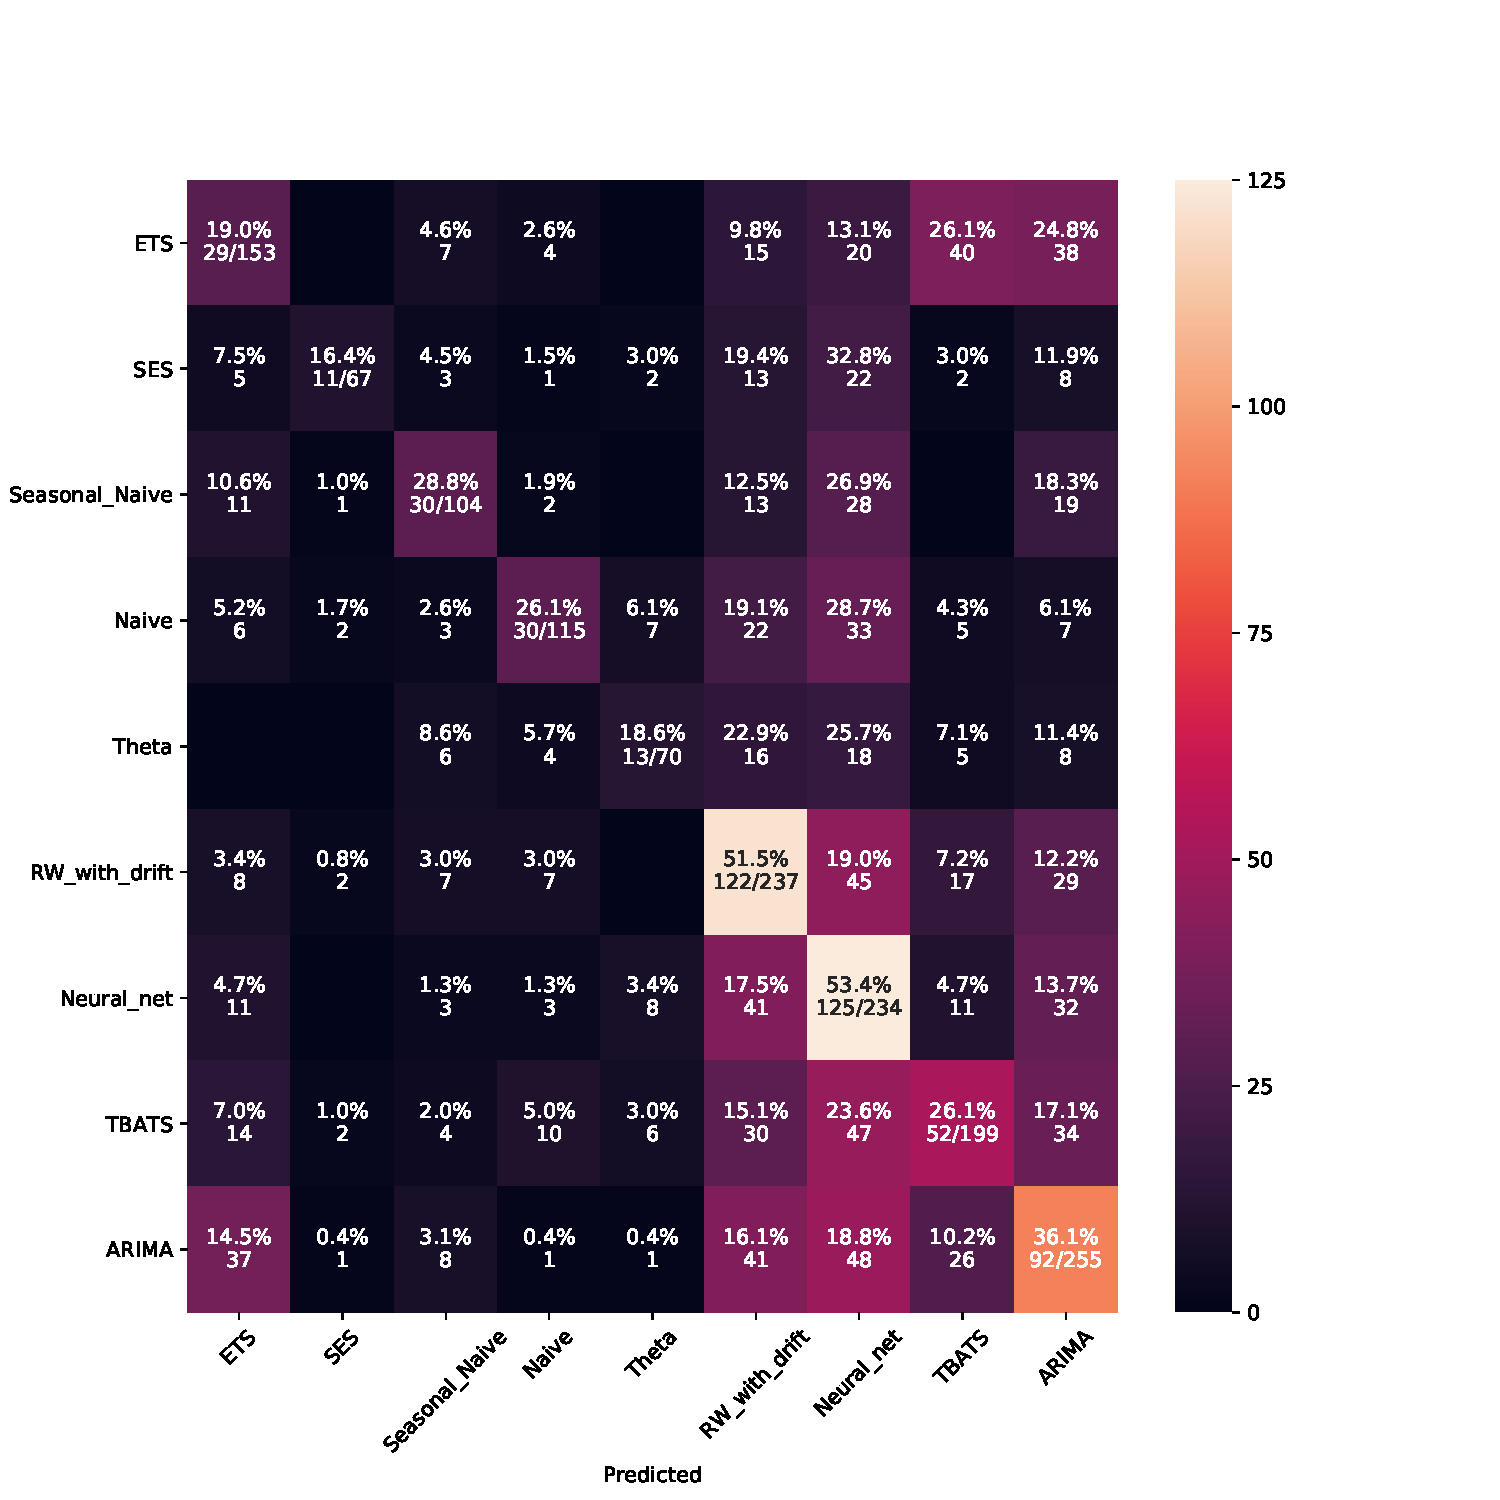
\includegraphics[width=
		0.9\textwidth]{conf}%{./Pictures/mainscreen1.png}
		\caption{Матрица ошибок алгоритма}
		\label{conf}
	\end{center}
\end{figure} 

На графике на Рис. \ref{conf} матрица ошибок наиболее эффективного варианта алгоритма на тестовых данных. Иные метрики качества можно найти в таблице на Рис. \ref{metrics}. Как можно увидеть, качество не идеальное. Будем честны с самими собой, оно не очень. Однако оно значительно выше просто случайного угадывания модели. Для модели с большим количеством классов такое поведение достаточно характерно. Есть несколько вариантов объяснения сложившейся ситуации:

\begin{enumerate}
	\item Недостаточный размер выборки. 
	
	Эта причина хотя и не слишком сильно заметна в данной работе, но всё же имеет место быть. Например, некоторые простые модели-победители (SES, Theta) представлены довольно скромным количеством наблюдений и выборка явно несбалансирована в пользу нейронной сети, ARIMA, TBATS и ETS. Сложно представить какой-то адекватный метод борьбы с дисбалансом кроме расширения исходной выборки временных рядов. Возможно, получилось бы частично решить эту проблему с помощью более активной генерации искуственных рядов.
	
	Смещение легко заметить и на матрице ошибок. Видно невооружённым глазом, что правая часть матрицы заметно теплее, чем левая. Это означает, что алгоритм склонен ошибаться в сторону более сложных моделей.
	
	
	\item Низкие различия между лейблами.
	
	Вполне возможен следующий вариант событий. Допустим, есть ряд с сильной сезонностью. В таком случае он должен относительно хорошо предсказываться и ETS, и TBATS, и ARIMA. Стало быть, разница в ошибке между условно тремя наилучшими алгоритмами может быть весьма мала. Cледовательно, алгоритм в любом случае может часто ошибаться на моделях с одинаковыми сильными сторонами.
	
	Это мы и можем заметить на матрице ошибок. Например, в первом ряду вместо ETS частенько предсказывались как раз TBATS или ARIMA. Аналогично относительно TBATS и ARIMA. Об этом свидетельствует существенно выделяющийся тёплый квадрат в правом нижнем углу. 
	
	\item Недостаточное количество элементов в ансамбле или необходимость более сильного алгоритма. 
	
	В данной работе использован случайный лес в основном из-за его простоты в настройке и малого количества подлежащих подбору гиперпараметров. Однако никто  не запрещает запустить кросс-валидацию на каком-нибудь градиентном бустинге, что, безусловно, займёт существенно больше времени. Пытливому читателю предлагается реализовать этот эксперимент самостоятельно.
	
\end{enumerate}

\newpage
\section{Заключение}

Подводя итоги данной работы, следует отметить что принцип мета-обучения представляет собой весьма интересный метод отбора моделей. Построенная в последней главе модель демонстрирует свою работоспособность несмотря на наличие некоторого количества необходимых доработок.

Также предварительный анализ мета-характеристик позволяет получить любопытные выводы относительно типизации признаков временных рядов. Например, можно вновь упомянуть склонность дневных рядов к нестационарности или высокую хаотичность годовых рядов. 

Тем не менее, модель имеет ряд ограничений. Например, необходимо тщательно подходить к отбору характеристик и  способу их обработки, а также к выбору пула моделей. К тому же, вполне возможно что даже при преодолении ряда проблем модель не сделает существенных прорывов по качеству классификации. Попросту неясно насколько может быть точна эта модель. Безусловно, в этой сфере необходимо продолжать исследования.	

\newpage
\section{Библиография}


	\begin{thebibliography}{99}
	\bibitem{visual} \href{https://www.researchgate.net/profile/Yanfei_Kang/publication/312449797_Visualising_forecasting_algorithm_performance_using_time_series_instance_spaces/links/5b03b9d8a6fdccf9e4f78451/Visualising-forecasting-algorithm-performance-using-time-series-instance-spaces.pdf}{Kang Y., Hyndman R. J., Smith-Miles K. Visualising forecasting algorithm performance using time series instance spaces //International Journal of Forecasting. – 2017. – Т. 33. – №. 2. – С. 345-358.} 
	\bibitem{start}
	\href{https://www.monash.edu/business/ebs/research/publications/ebs/wp06-2018.pdf}{Talagala T. S. et al. Meta-learning how to forecast time series. – Monash University, Department of Econometrics and Business Statistics, 2018. – №. 6/18.}
	\bibitem{pca}
	\href{https://forecasters.org/wp-content/uploads/gravity_forms/7-2a51b93047891f1ec3608bdbd77ca58d/2013/07/Widodo_Agus_ISF2013.pdf}{Widodo, A \& I Budi (2013). “Model selection using dimensionality reduction of time series
		characteristics”. Paper presented at the International Symposium on Forecasting, Seoul,
		South Korea. June 2013.}

	
	\bibitem{meta}
	\href{http://citeseerx.ist.psu.edu/viewdoc/download?doi=10.1.1.111.2000&rep=rep1&type=pdf}{Wang X., Smith-Miles K., Hyndman R. Rule induction for forecasting method selection: Meta-learning the characteristics of univariate time series //Neurocomputing. – 2009. – Т. 72. – №. 10-12. – С. 2581-2594.}

	
	\bibitem{neural}
	\href{https://www.researchgate.net/profile/Sven_Crone/publication/301549075_Meta-Learning_with_Neural_Networks_and_Landmarking_for_Forecasting_Model_Selection_-_An_Empirical_Evaluation_of_Different_Feature_Sets_Applied_to_Industry_Data/links/5a8d8a6eaca272c56bc30fba/Meta-Learning-with-Neural-Networks-and-Landmarking-for-Forecasting-Model-Selection-An-Empirical-Evaluation-of-Different-Feature-Sets-Applied-to-Industry-Data.pdf}{Kück M., Crone S. F., Freitag M. Meta-learning with neural networks and landmarking for forecasting model selection an empirical evaluation of different feature sets applied to industry data //2016 International Joint Conference on Neural Networks (IJCNN). – IEEE, 2016. – С. 1499-1506.
}
	
	
	\bibitem{anomalous}
		\href{https://robjhyndman.com/papers/icdm2015.pdf}{	Hyndman R. J., Wang E., Laptev N. Large-scale unusual time series detection //2015 IEEE international conference on data mining workshop (ICDMW). – IEEE, 2015. – С. 1616-1619.}
		
	\bibitem{chaos}
	\href{https://arxiv.org/pdf/0906.1418.pdf}{Gottwald G. A., Melbourne I. On the implementation of the 0–1 test for chaos //SIAM Journal on Applied Dynamical Systems. – 2009. – Т. 8. – №. 1. – С. 129-145.}
	
	\bibitem{frac}
	\href{https://www.jstor.org/stable/pdf/2347679.pdf?casa_token=IHbWtz1Mt3gAAAAA:jzPs29XzT4MV4R1rqL1SgF7RP1QdIKFJLluogM-LmyhQrOFTf2zv6_gz-rvOdTORp5FVU7x-3tTxAOqs6PXgSwEGFRsOcW7dHP8AEKxDVq16_ywZJ4YS}{Haslett J., Raftery A. E. Space‐time modelling with long‐memory dependence: Assessing Ireland's wind power resource //Journal of the Royal Statistical Society: Series C (Applied Statistics). – 1989. – Т. 38. – №. 1. – С. 1-21.}
	
	\bibitem{nonlin}
	\href{https://onlinelibrary.wiley.com/doi/pdf/10.1111/j.1467-9892.1993.tb00139.x?casa_token=VTgIjr6WkKwAAAAA:INpZkev855M5upMdwOsxh7gSAU0ZRRItxCqwtTFNg7Dn5LVV-RrrWZ9f4Ob3ECcnRytZOLM1vElakl93}{Teräsvirta T., Lin C. F., Granger C. W. J. Power of the neural network linearity test //Journal of time series analysis. – 1993. – Т. 14. – №. 2. – С. 209-220.}

	\bibitem{tsay}
	\href{http://citeseerx.ist.psu.edu/viewdoc/download?doi=10.1.1.665.8479&rep=rep1&type=pdf}{Tsay R. S. Analysis of financial time series. – John wiley \& sons, 2005. – Т. 543.}
	
	\bibitem{ets}
	\href{https://books.google.ru/books?hl=ru&lr=&id=GSyzox8Lu9YC&oi=fnd&pg=PA2&ots=1q8pJKrEn6&sig=tZEeP-DbxVTkxZ-EfNVDQ9njYWs&redir_esc=y#v=onepage&q&f=false}{Hyndman R. et al. Forecasting with exponential smoothing: the state space approach. – Springer Science \& Business Media, 2008.}
	
	\bibitem{theta}
	\href{https://www.researchgate.net/profile/Vassilis_Assimakopoulos/publication/223049702_The_theta_model_A_decomposition_approach_to_forecasting/links/5a7e3b2daca272a73765ccf8/The-theta-model-A-decomposition-approach-to-forecasting.pdf}{Assimakopoulos V., Nikolopoulos K. The theta model: a decomposition approach to forecasting //International journal of forecasting. – 2000. – Т. 16. – №. 4. – С. 521-530.}
	\bibitem{arima}
	Khandakar Y., Hyndman R. J. Automatic time series forecasting: the forecast Package for R //Journal of Statistical Software. – 2008. – Т. 27. – №. 03.
	
	\bibitem{nnet}
	\href{http://citeseerx.ist.psu.edu/viewdoc/download?doi=10.1.1.115.140&rep=rep1&type=pdf}{Zhang G. P. Business forecasting with artificial neural networks: An overview //Neural networks in business forecasting. – IGI Global, 2004. – С. 1-22.}
	
	\bibitem{smape}
	\href{https://pdfs.semanticscholar.org/385c/dea69e2c0f8a39e9f8420b326f91a9e7019f.pdf}{Chen Z., Yang Y. Assessing forecast accuracy measures //Preprint Series. – 2004. – Т. 2010. – С. 2004-10. 	}
\end{thebibliography}


\newpage
\section{Приложения}

\subsection{Приложение 1}
\label{prcomp}
\begin{tabular}{|
		>{\columncolor[HTML]{91FF91}}l |l|l|}
	\hline
	\textbf{Характеристика} & \cellcolor[HTML]{91FF91}\textbf{PC1} & \cellcolor[HTML]{91FF91}\textbf{PC2} \\ \hline
	\textbf{x\_acf1} & -0.16426 & 0.117391 \\ \hline
	\textbf{diff1\_acf1} & -0.05932 & 0.17474 \\ \hline
	\textbf{diff2\_acf1} & -0.01464 & 0.038579 \\ \hline
	\textbf{x\_pacf5} & -0.16719 & -0.03532 \\ \hline
	\textbf{entropy} & 0.446646 & -0.14787 \\ \hline
	\textbf{lumpiness} & 0.013596 & -0.00819 \\ \hline
	\textbf{stability} & -0.1565 & 0.411073 \\ \hline
	\textbf{crossing\_points} & 0.022067 & -0.1291 \\ \hline
	\textbf{hurst} & -0.12943 & 0.12082 \\ \hline
	\textbf{unitroot\_kpss} & -0.30763 & 0.014806 \\ \hline
	\textbf{nonlinearity} & 0.027627 & 0.036854 \\ \hline
	\textbf{kurtosis} & 0.008388 & -0.00711 \\ \hline
	\textbf{skewness} & 0.018737 & -0.00821 \\ \hline
	\textbf{chaos} & 0.742364 & 0.19377 \\ \hline
	\textbf{lshift} & 0.107129 & 0.069215 \\ \hline
	\textbf{fspots} & -0.05229 & 0.013367 \\ \hline
	\textbf{max\_kl} & -0.00019 & 1.07E-05 \\ \hline
	\textbf{extreme\_dist\_shape} & 0.007313 & 0.004582 \\ \hline
	\textbf{seasonal\_strength} & -0.06556 & -0.81156 \\ \hline
	\textbf{trend} & -0.17425 & 0.164298 \\ \hline
	\textbf{spike} & 0.011608 & -0.00311 \\ \hline
	\textbf{linearity} & -0.06269 & -0.03019 \\ \hline
	\textbf{curvature} & 0.003 & 0.000864 \\ \hline
\end{tabular}

\newpage
\subsection{Приложение 2}
\label{strength}
\begin{figure}[!h]

\begin{center}
 	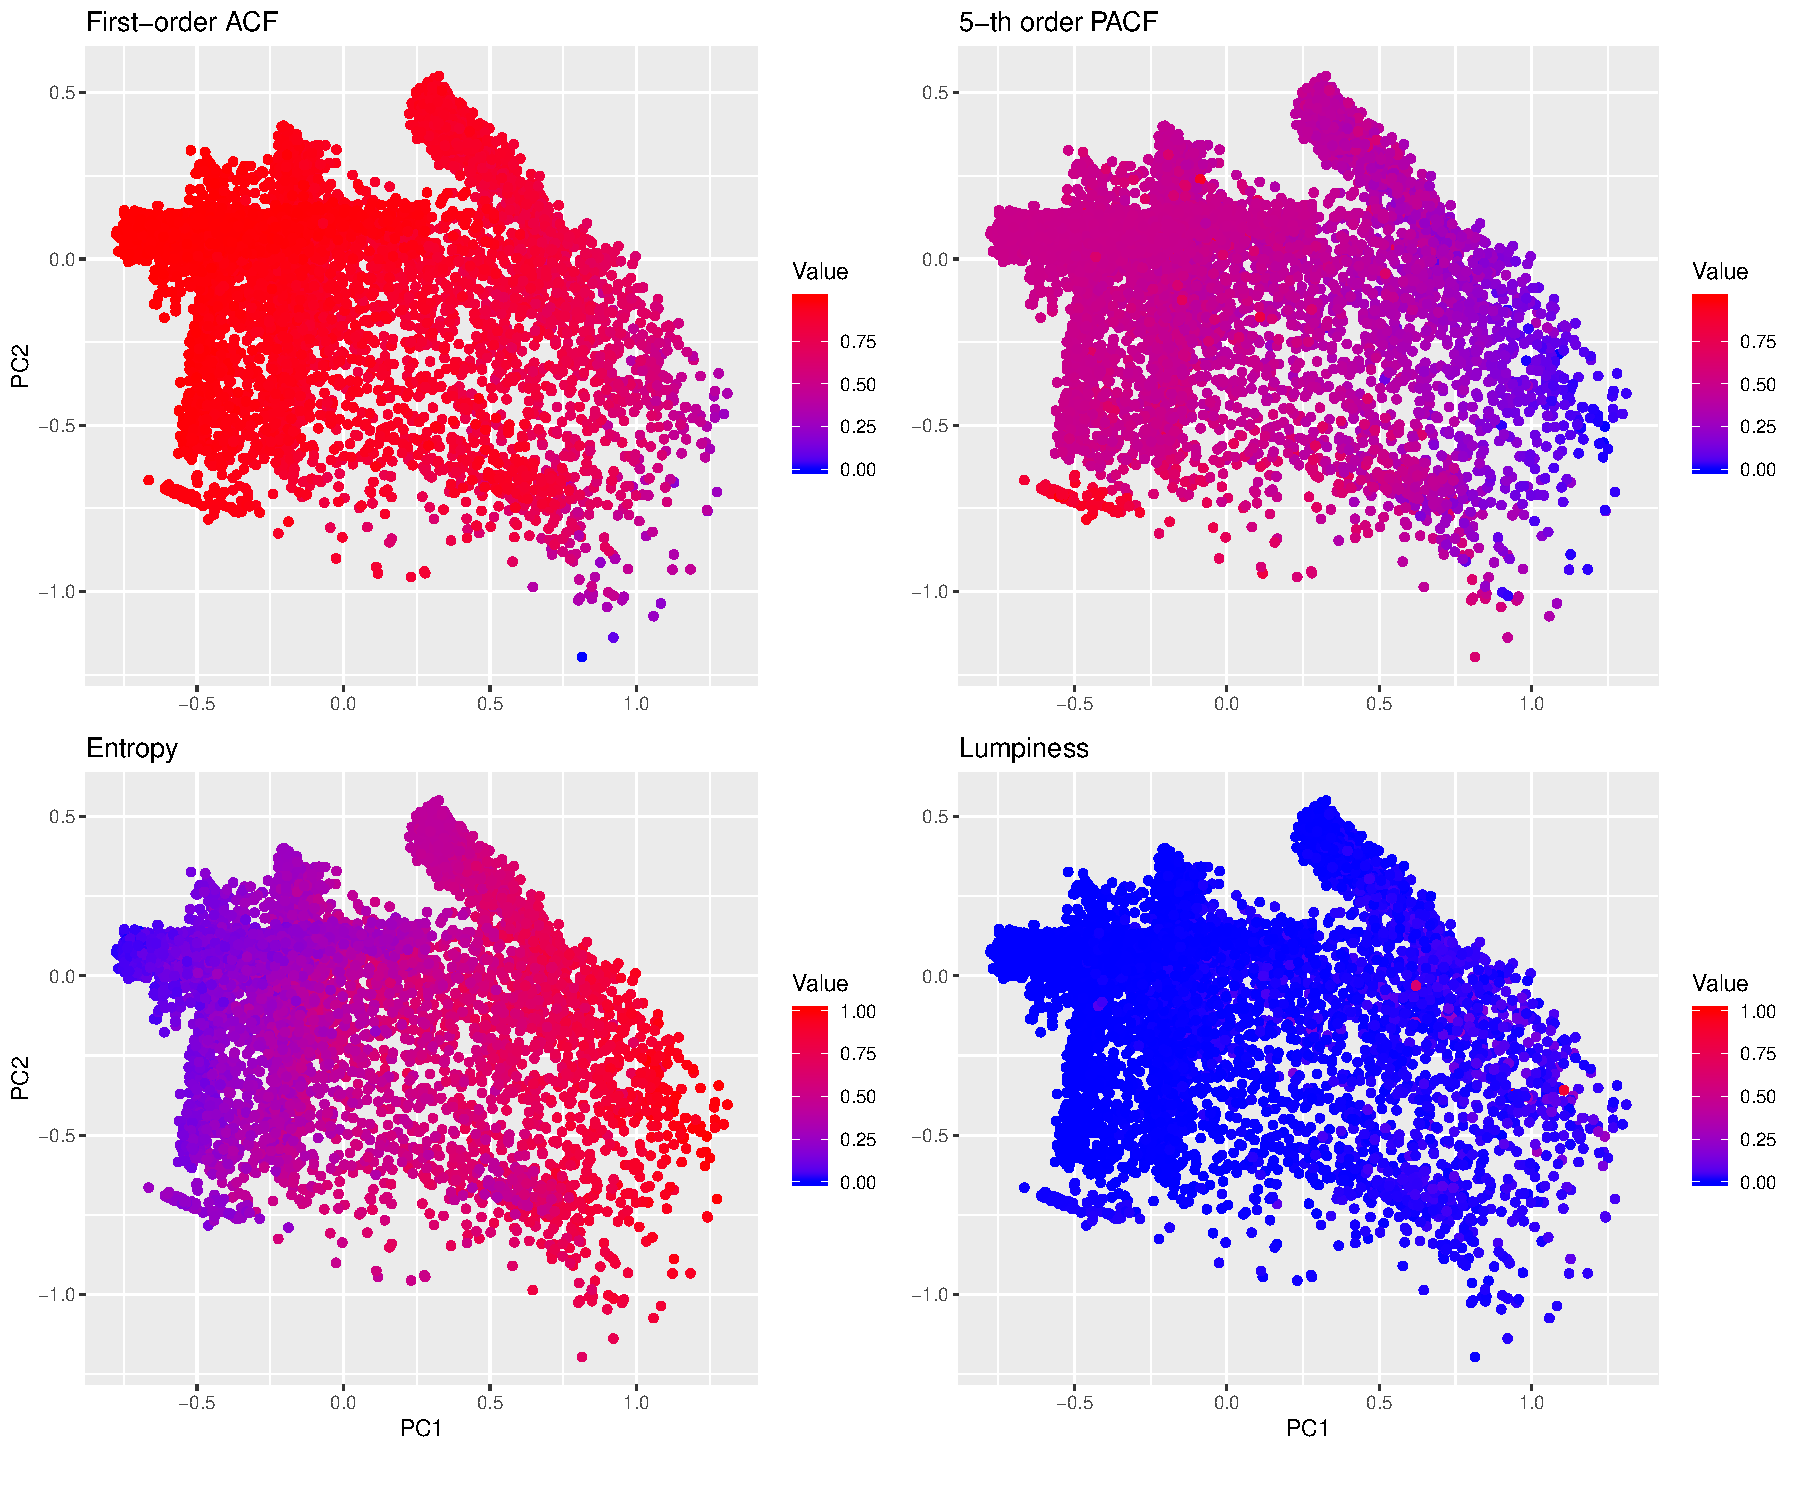
\includegraphics[width=0.8
 	\textwidth]{str_1}%{./Pictures/mainscreen1.png}

 	
 	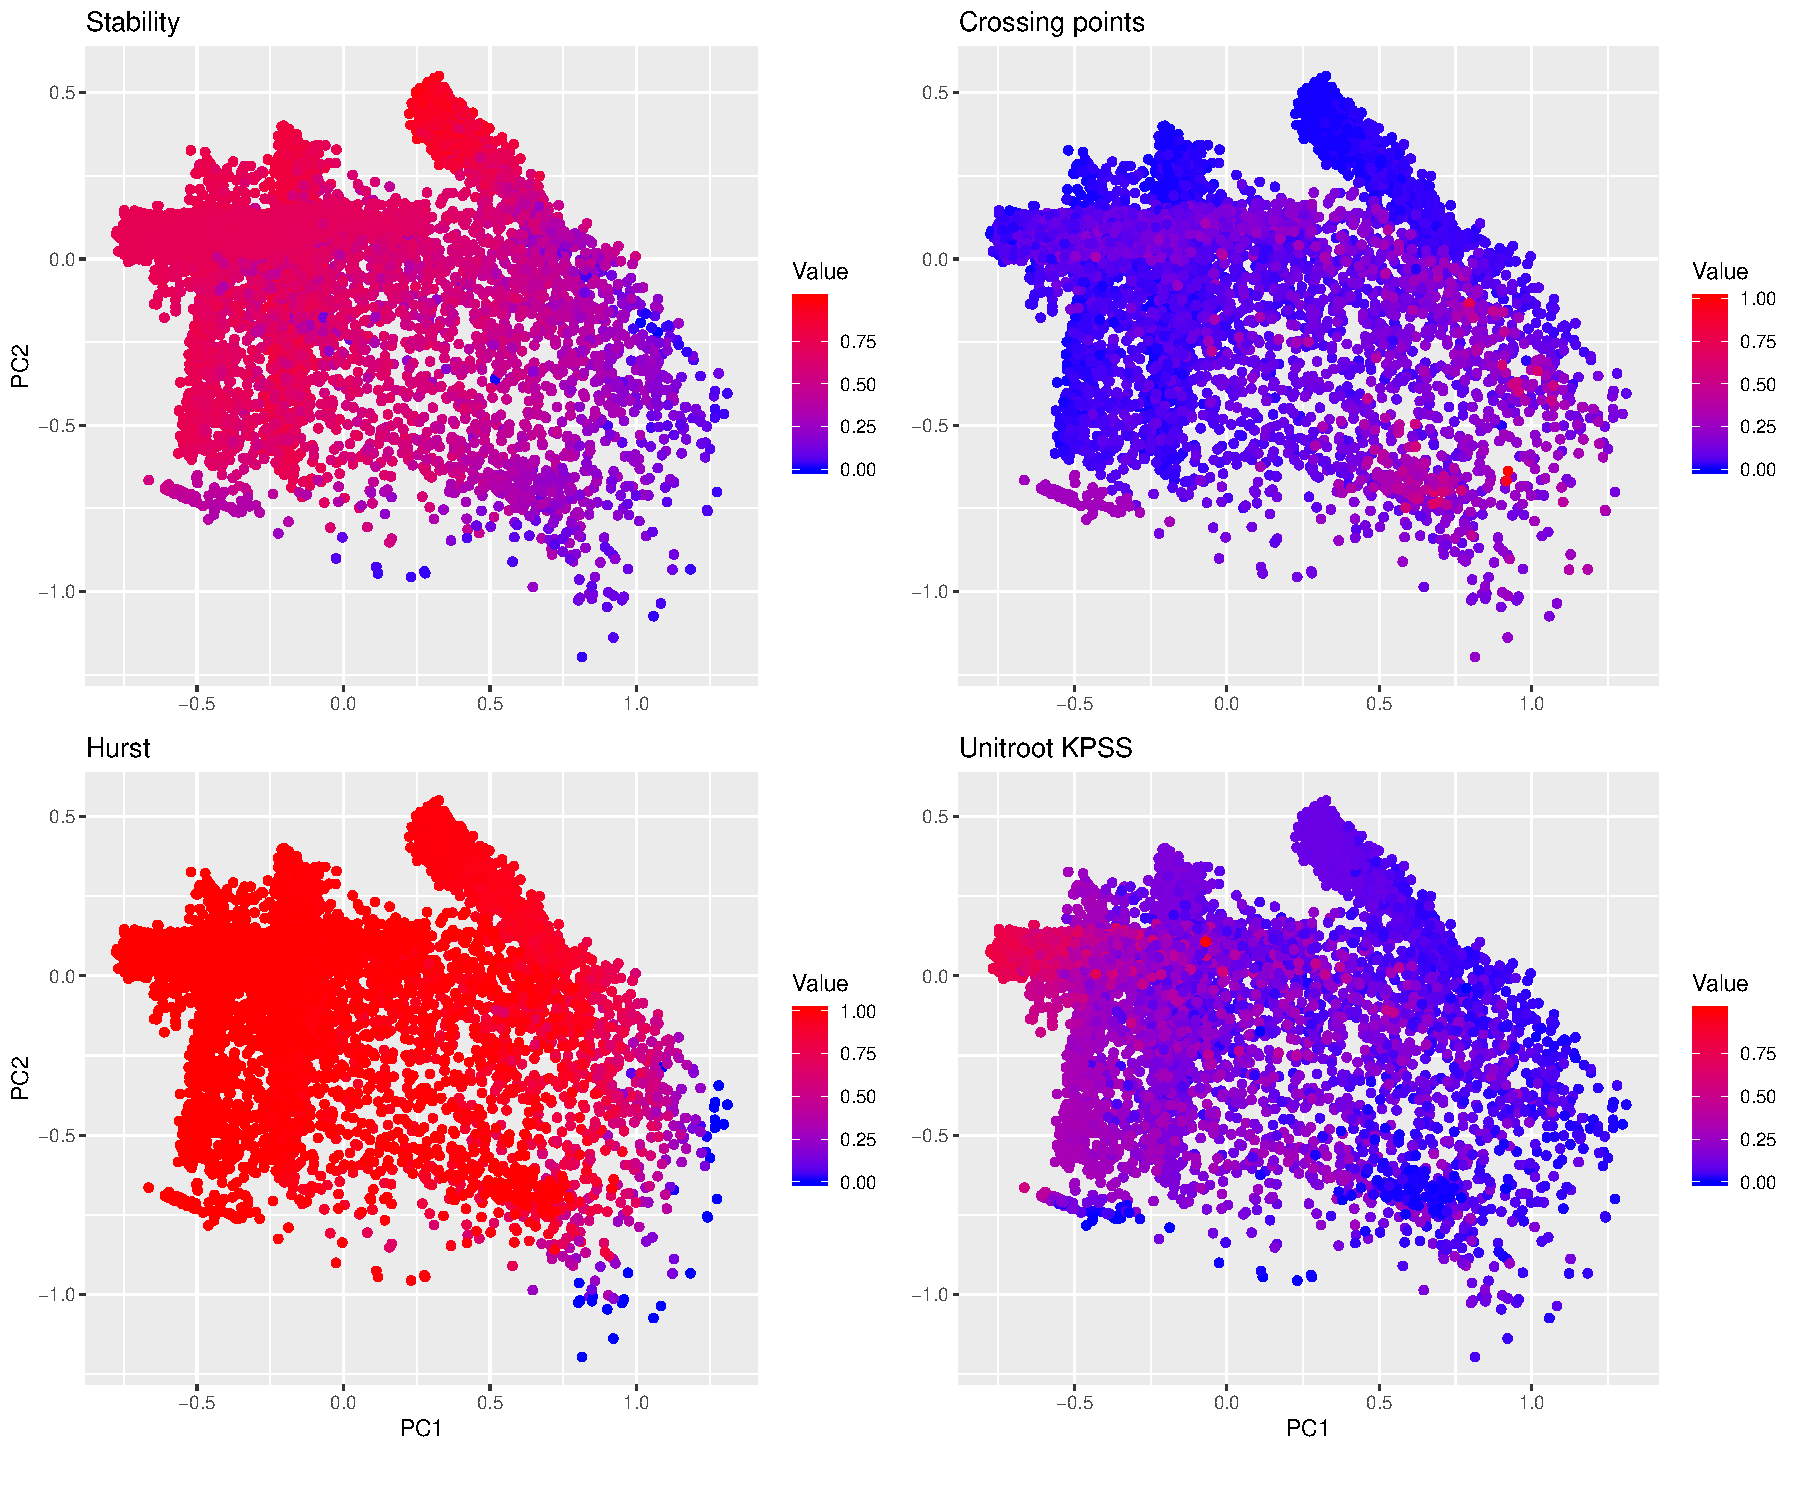
\includegraphics[width=0.8
 	\textwidth]{str_2}%{./Pictures/mainscreen1.png}
\end{center}

\end{figure} 
 
 
 \newpage
 \begin{figure}[!h]
 	
 	\begin{center}
 		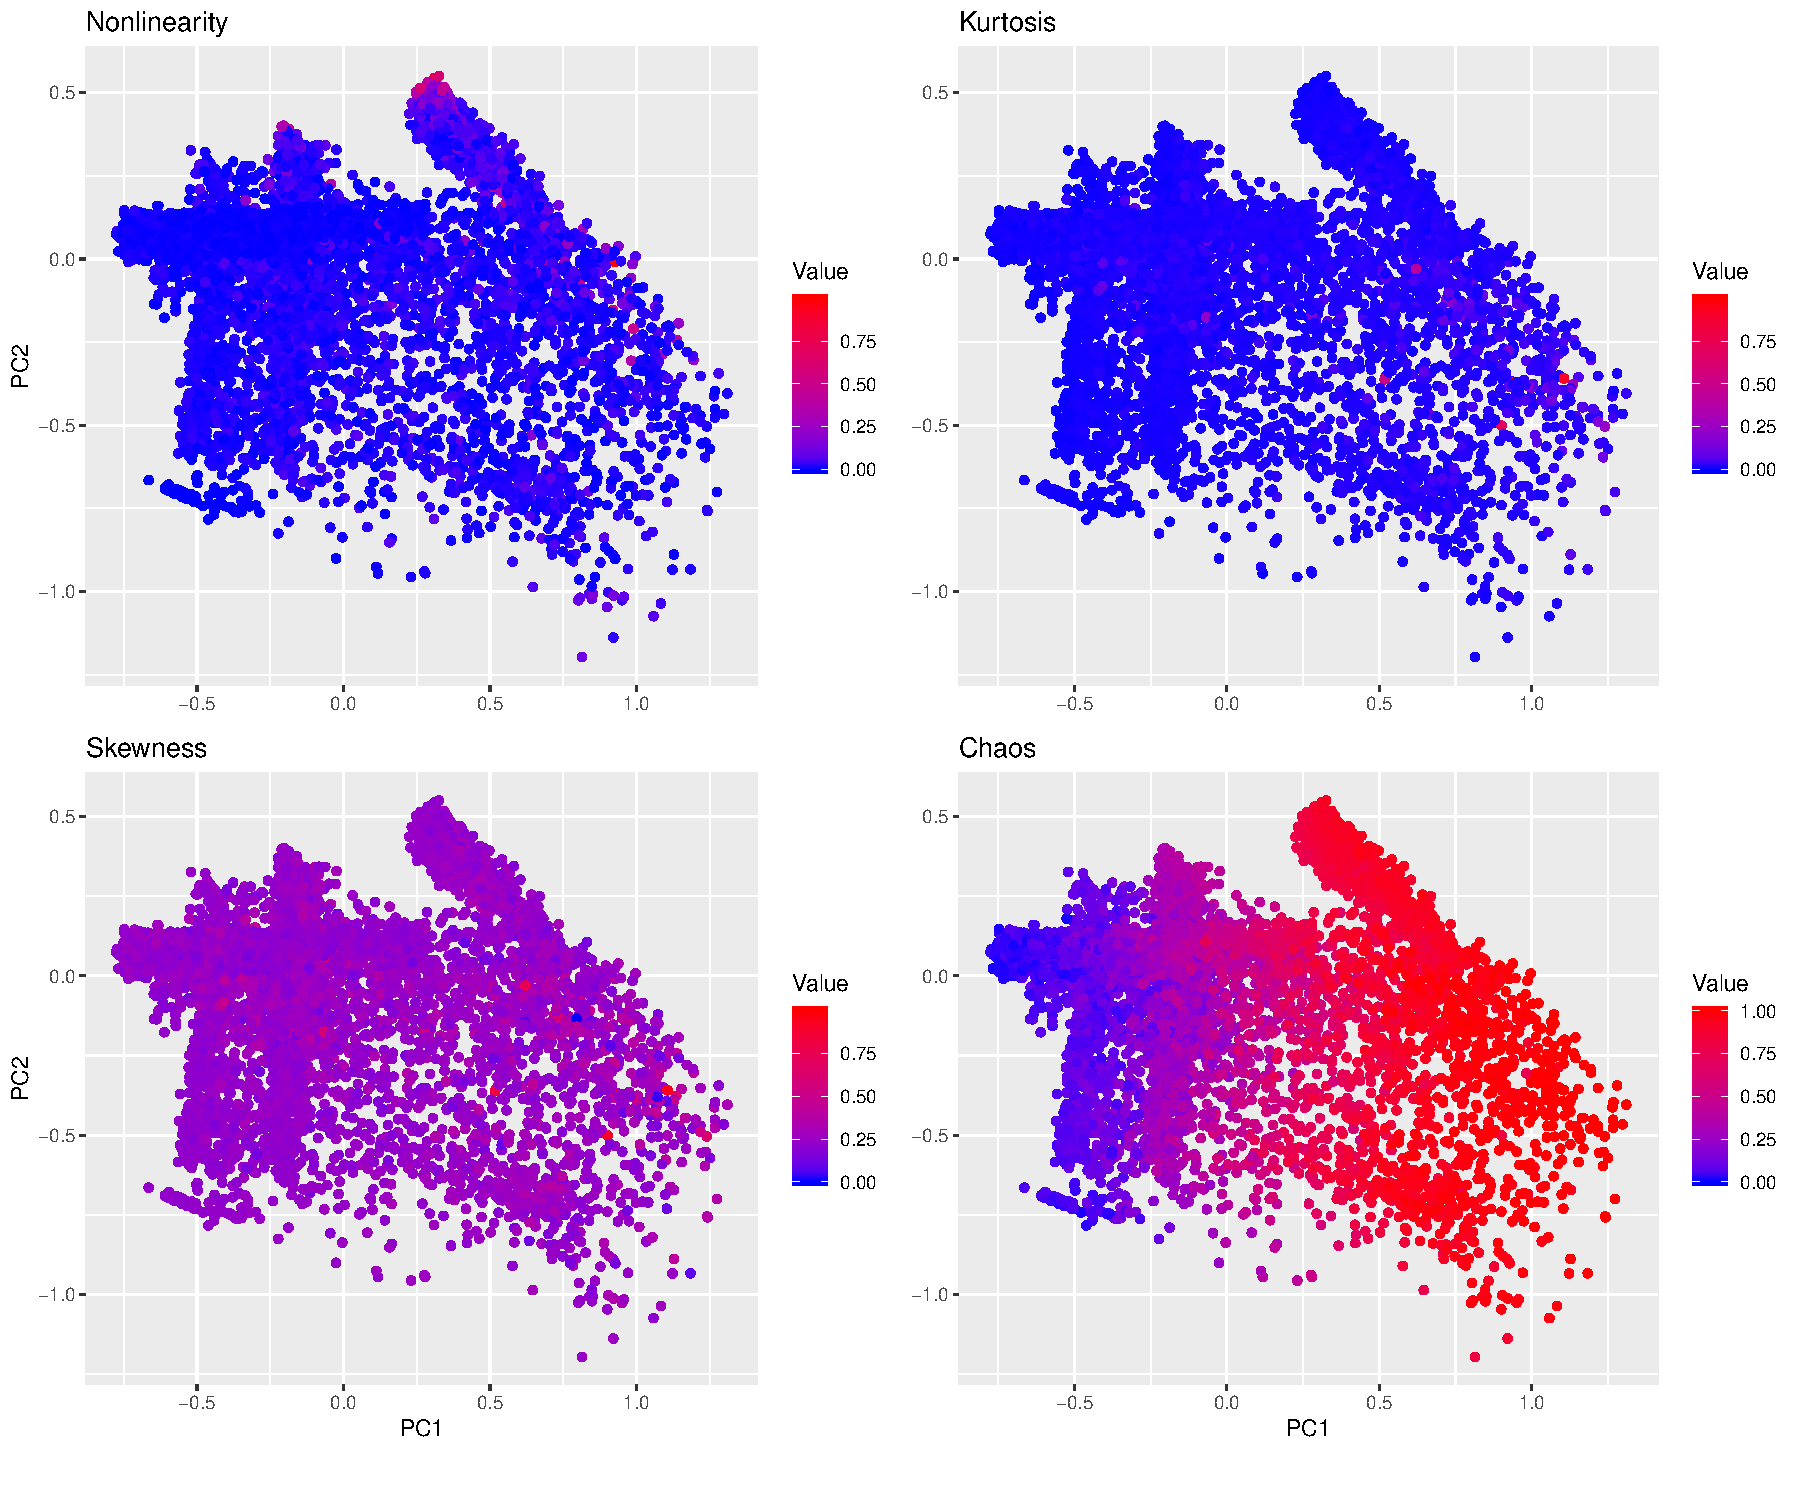
\includegraphics[width=0.7
 		\textwidth]{str_3}%{./Pictures/mainscreen1.png}
 		
 		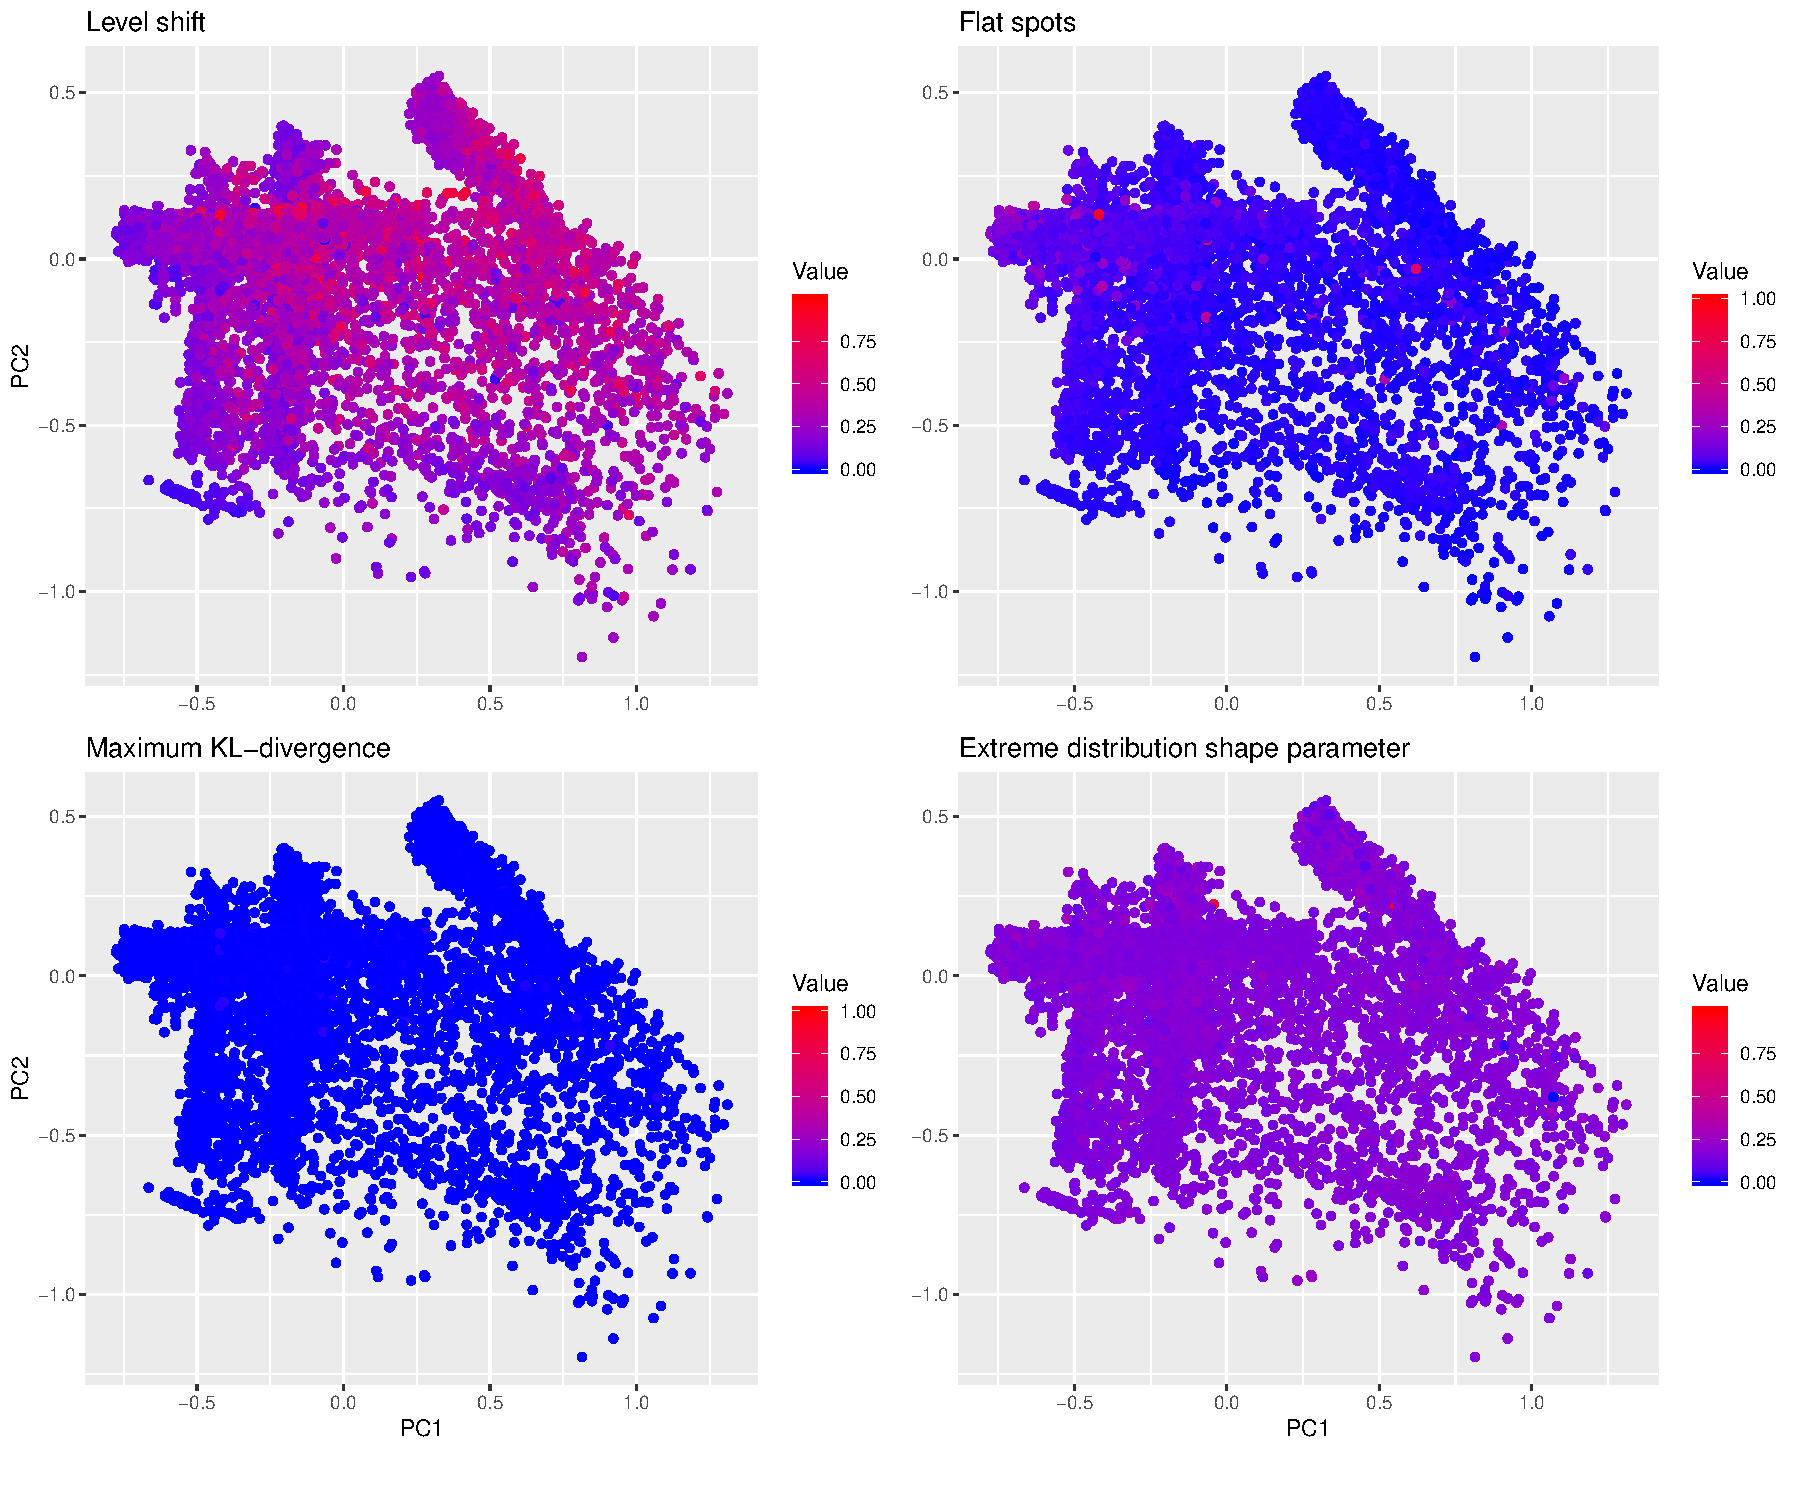
\includegraphics[width=0.8
 		\textwidth]{str_4}%{./Pictures/mainscreen1.png}
 	\end{center}
 	
 	
 \end{figure} 
	
\newpage

\begin{figure}[!h]
	
	\begin{center}
		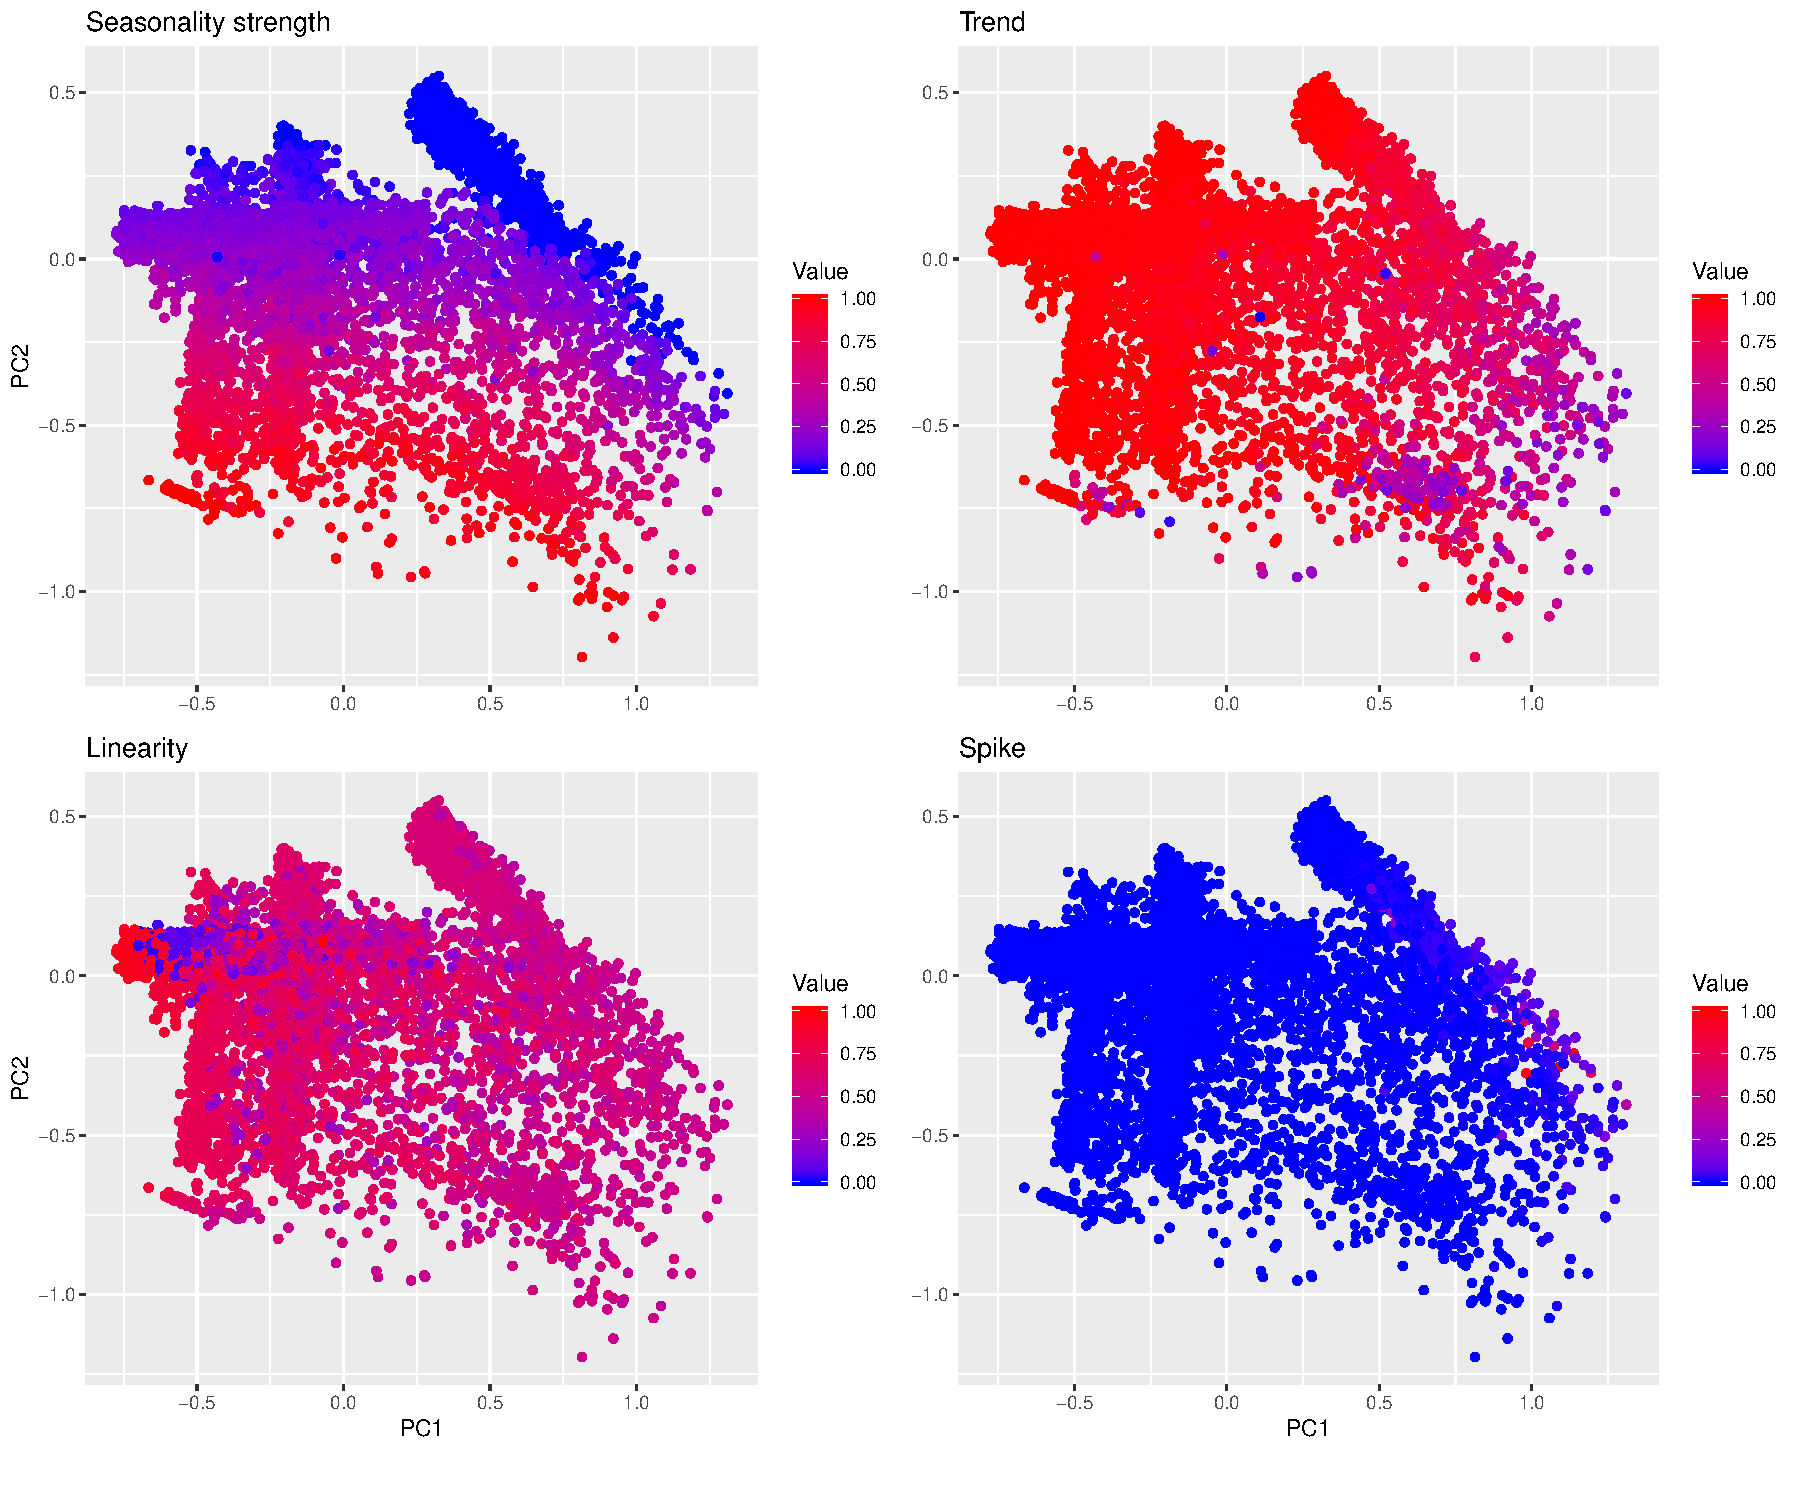
\includegraphics[width=0.8
		\textwidth]{str_5}%{./Pictures/mainscreen1.png}

		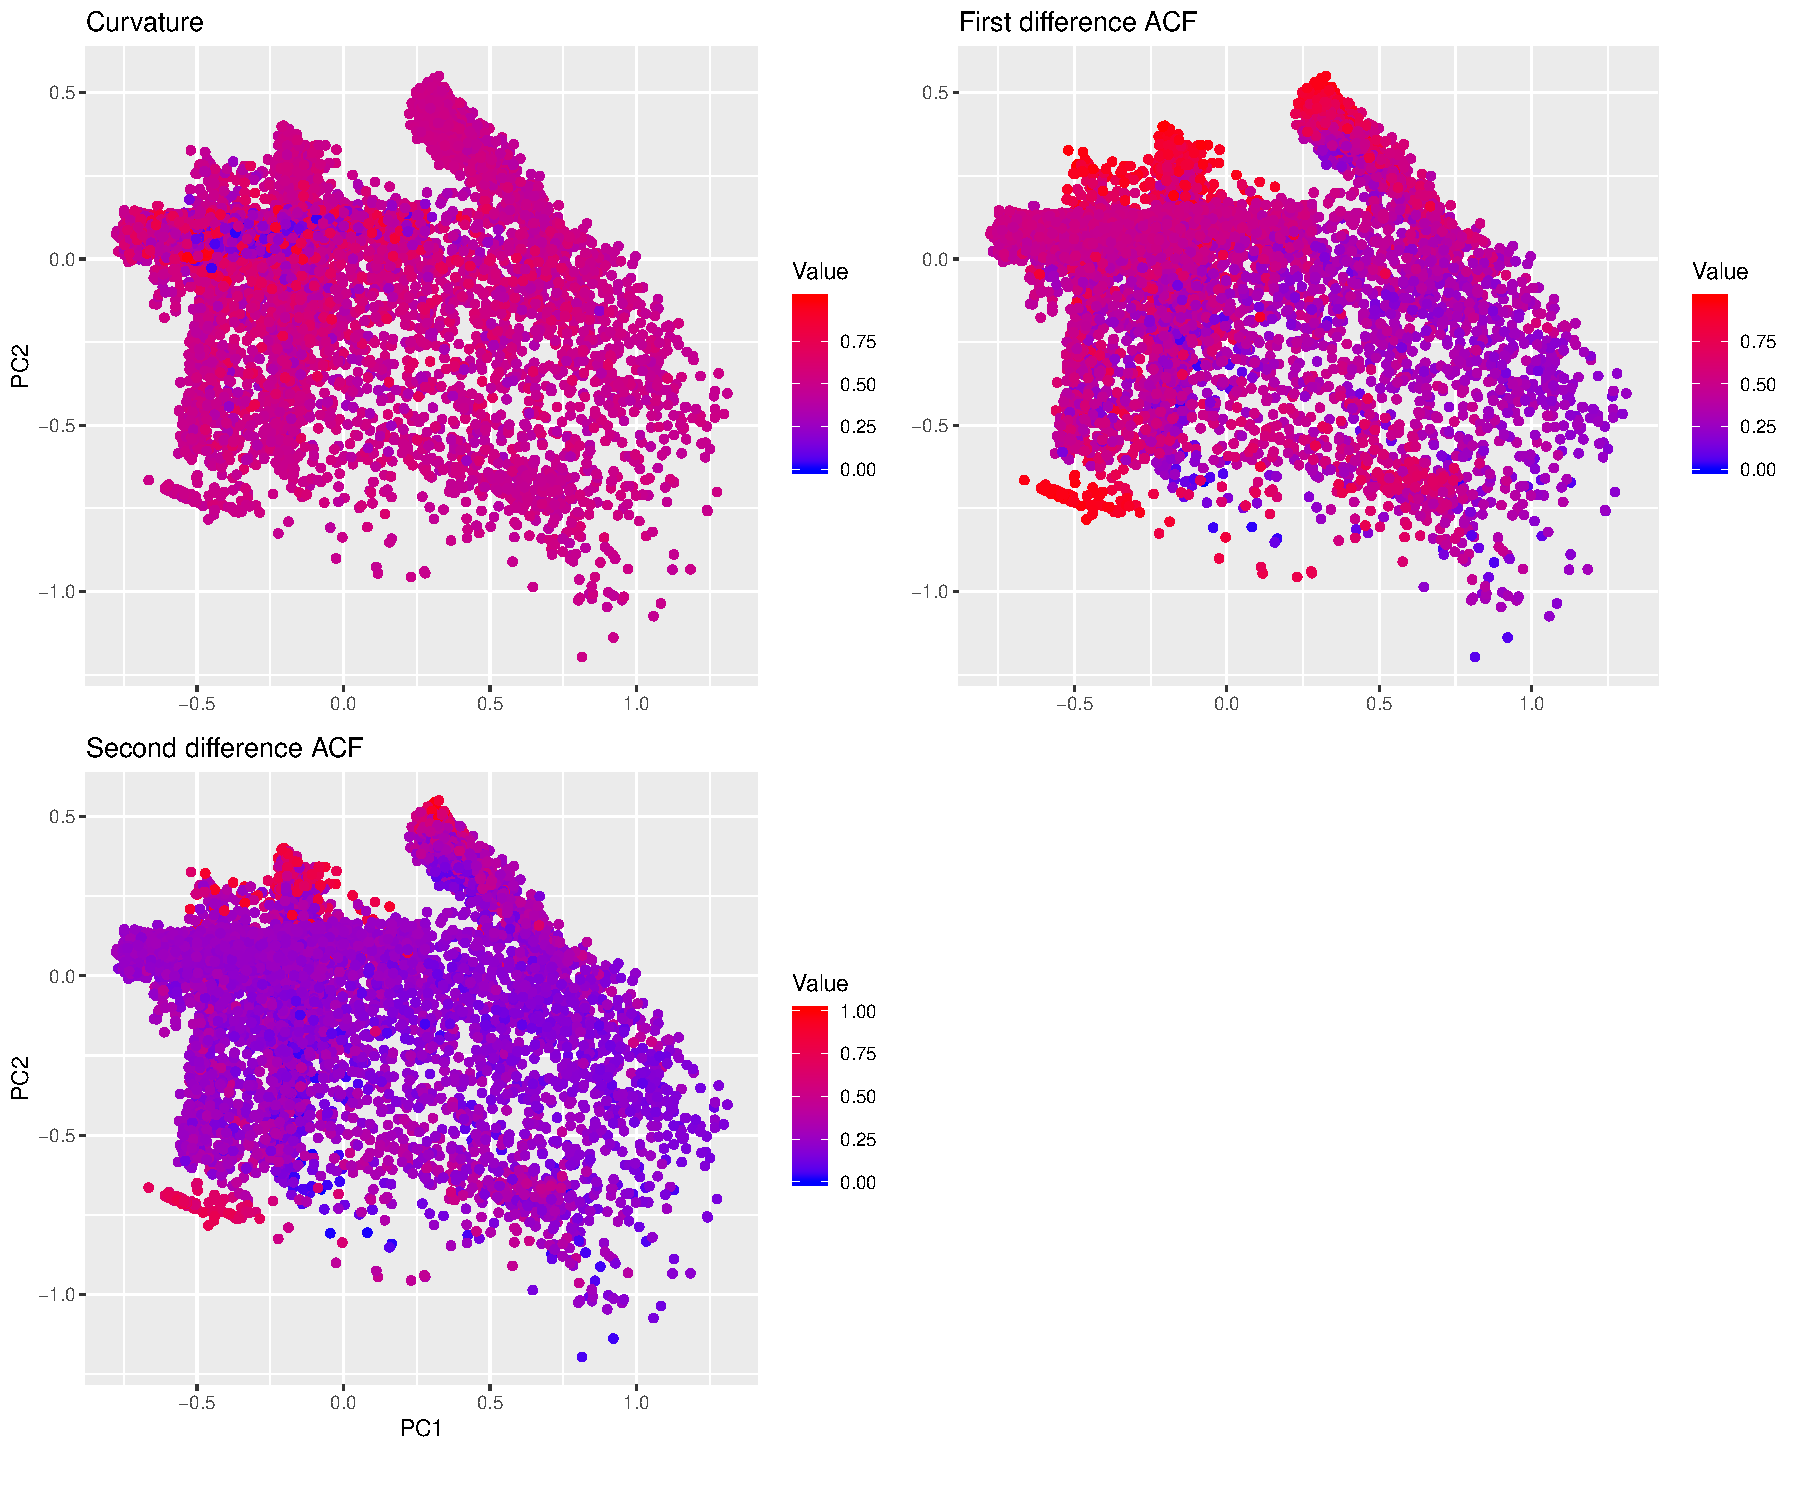
\includegraphics[width=0.8
		\textwidth]{str_6}%{./Pictures/mainscreen1.png}

	\end{center}
	
	
\end{figure} 


\newpage
\subsection{Приложение 3} 
\label{all_gen}
\begin{figure}[!h]
	
	\begin{center}
		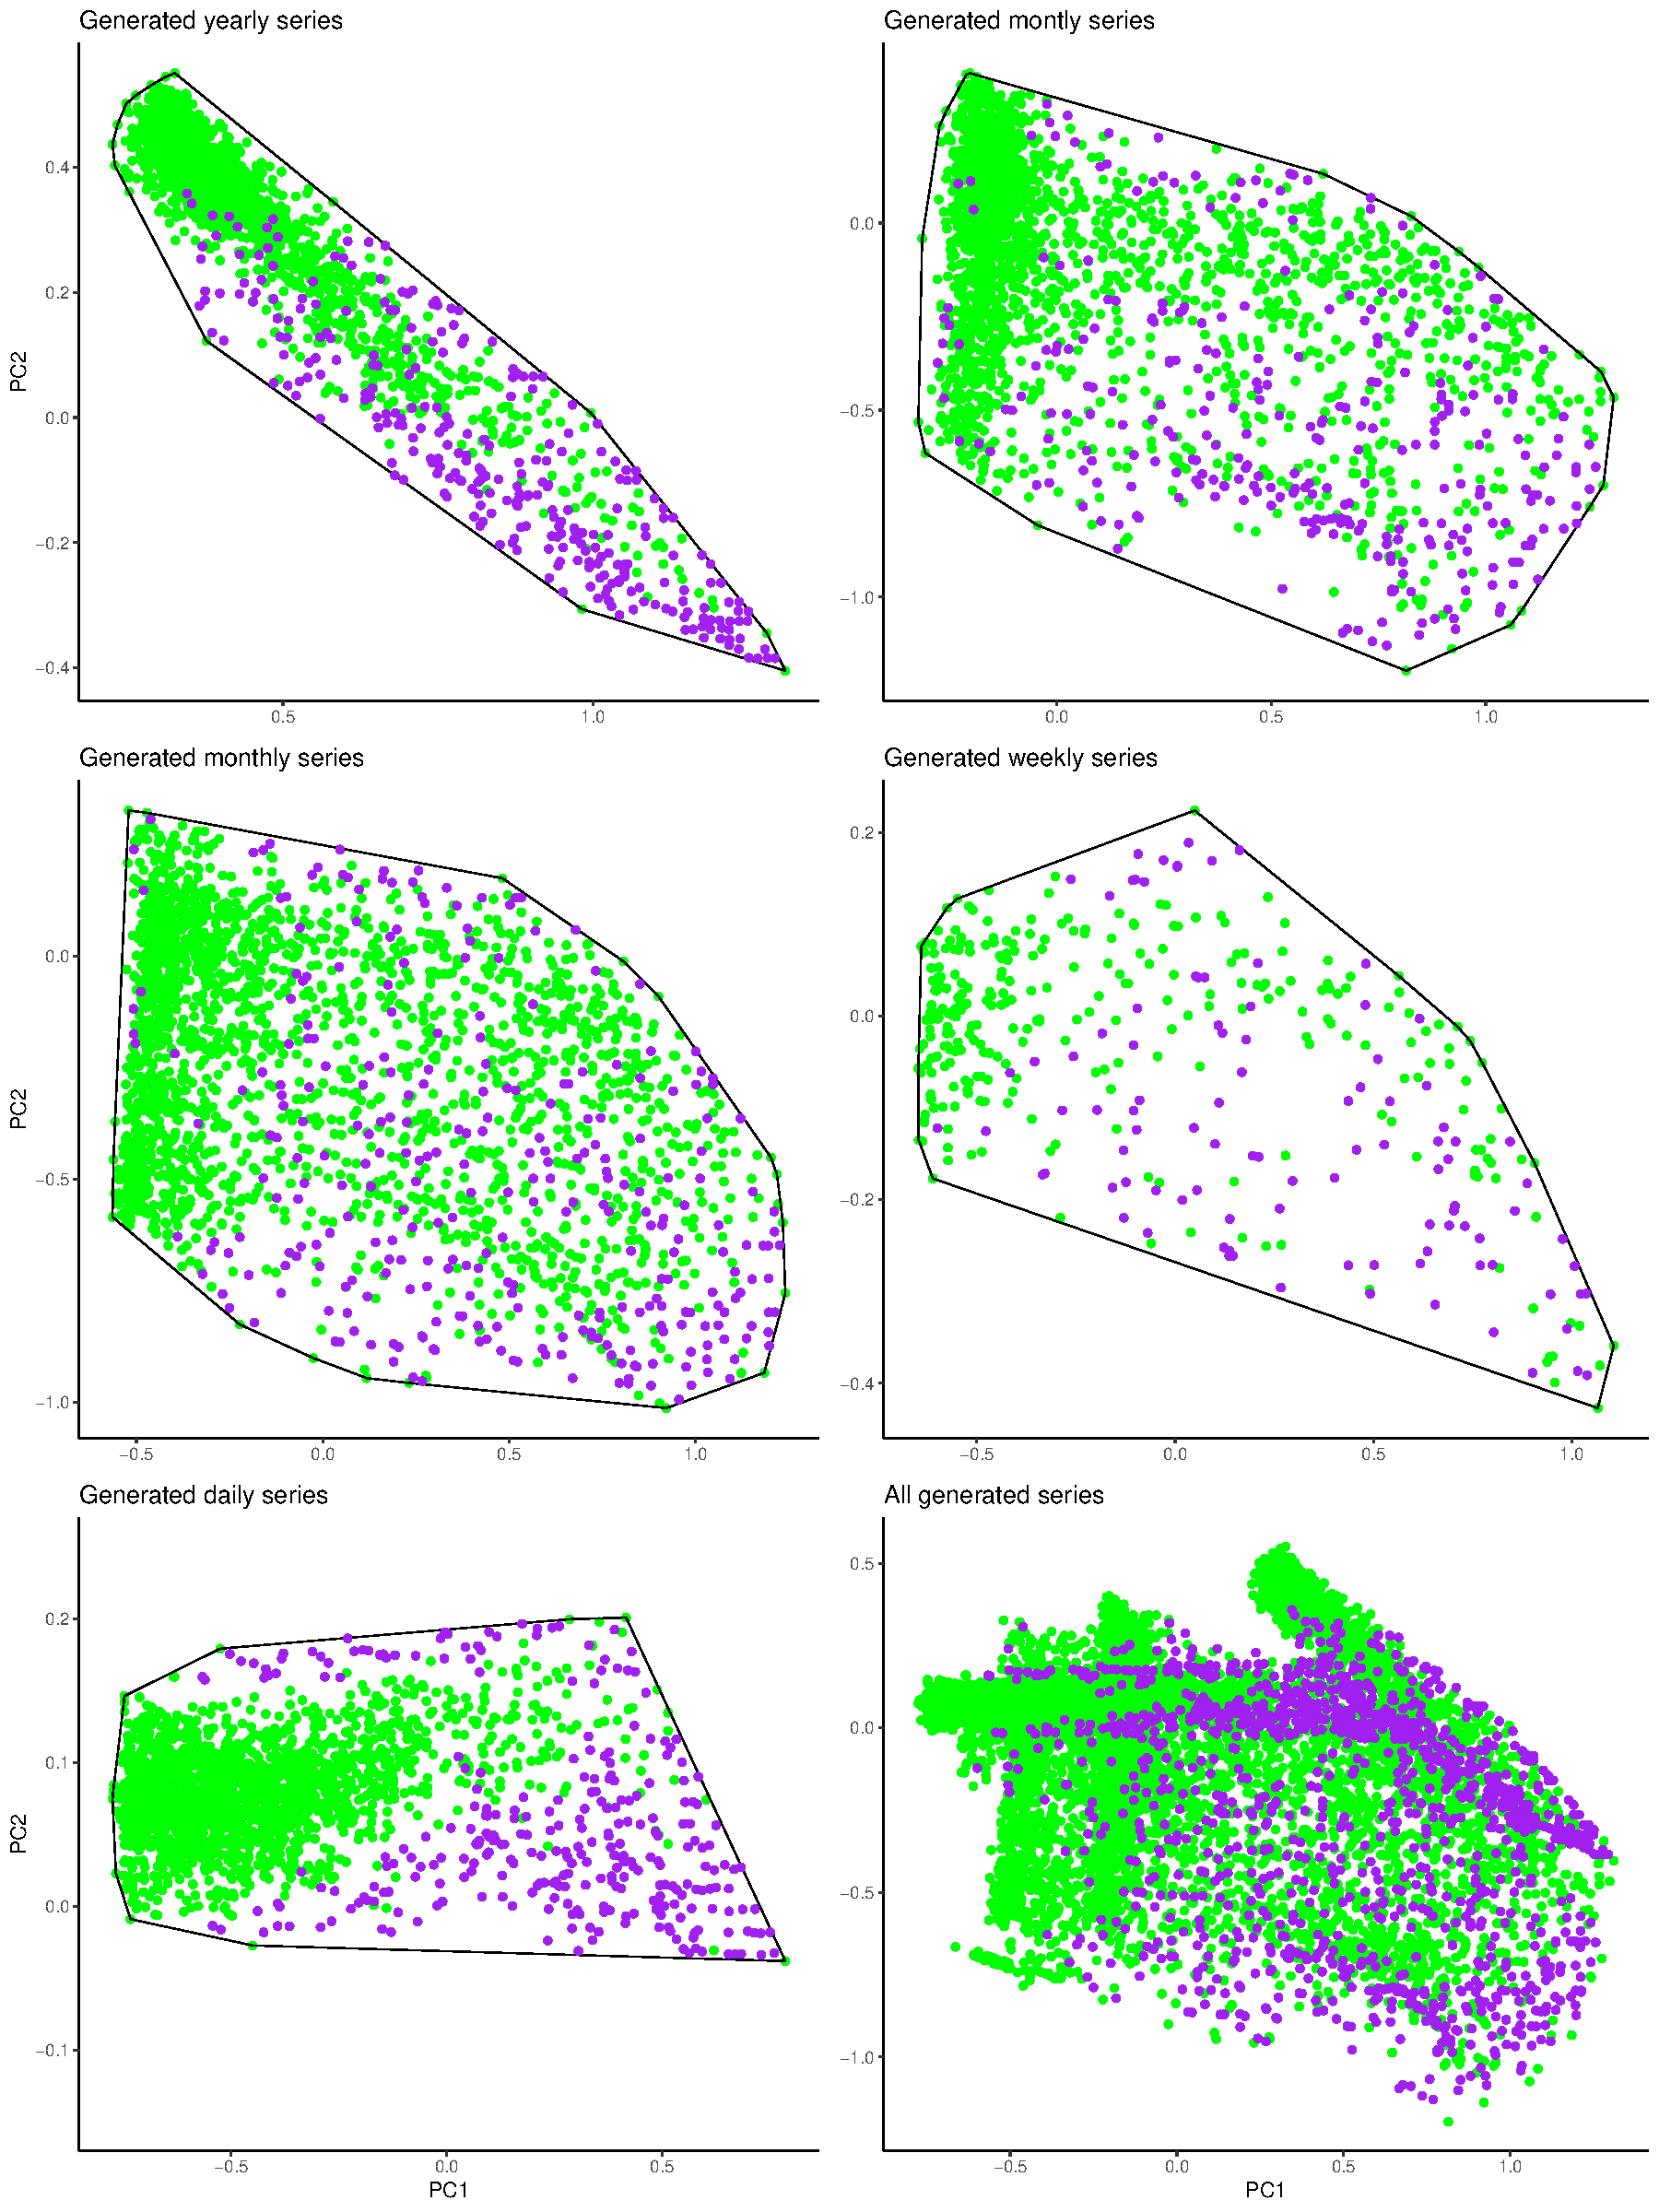
\includegraphics[width=
		\textwidth]{all_gen}%{./Pictures/mainscreen1.png}

	\end{center}
	
	
\end{figure} 

\newpage
\subsection{Приложение 4} 
\label{smape}
\begin{figure}[!h]
	\animategraphics[autoplay,controls,loop,scale=1,width=\textwidth]{1}{image}{1}{9}
\end{figure}


\newpage
\subsection{Приложение 5}

%#91ff91


\label{min_smape}
\begin{figure}[!h]
	
	\begin{center}
		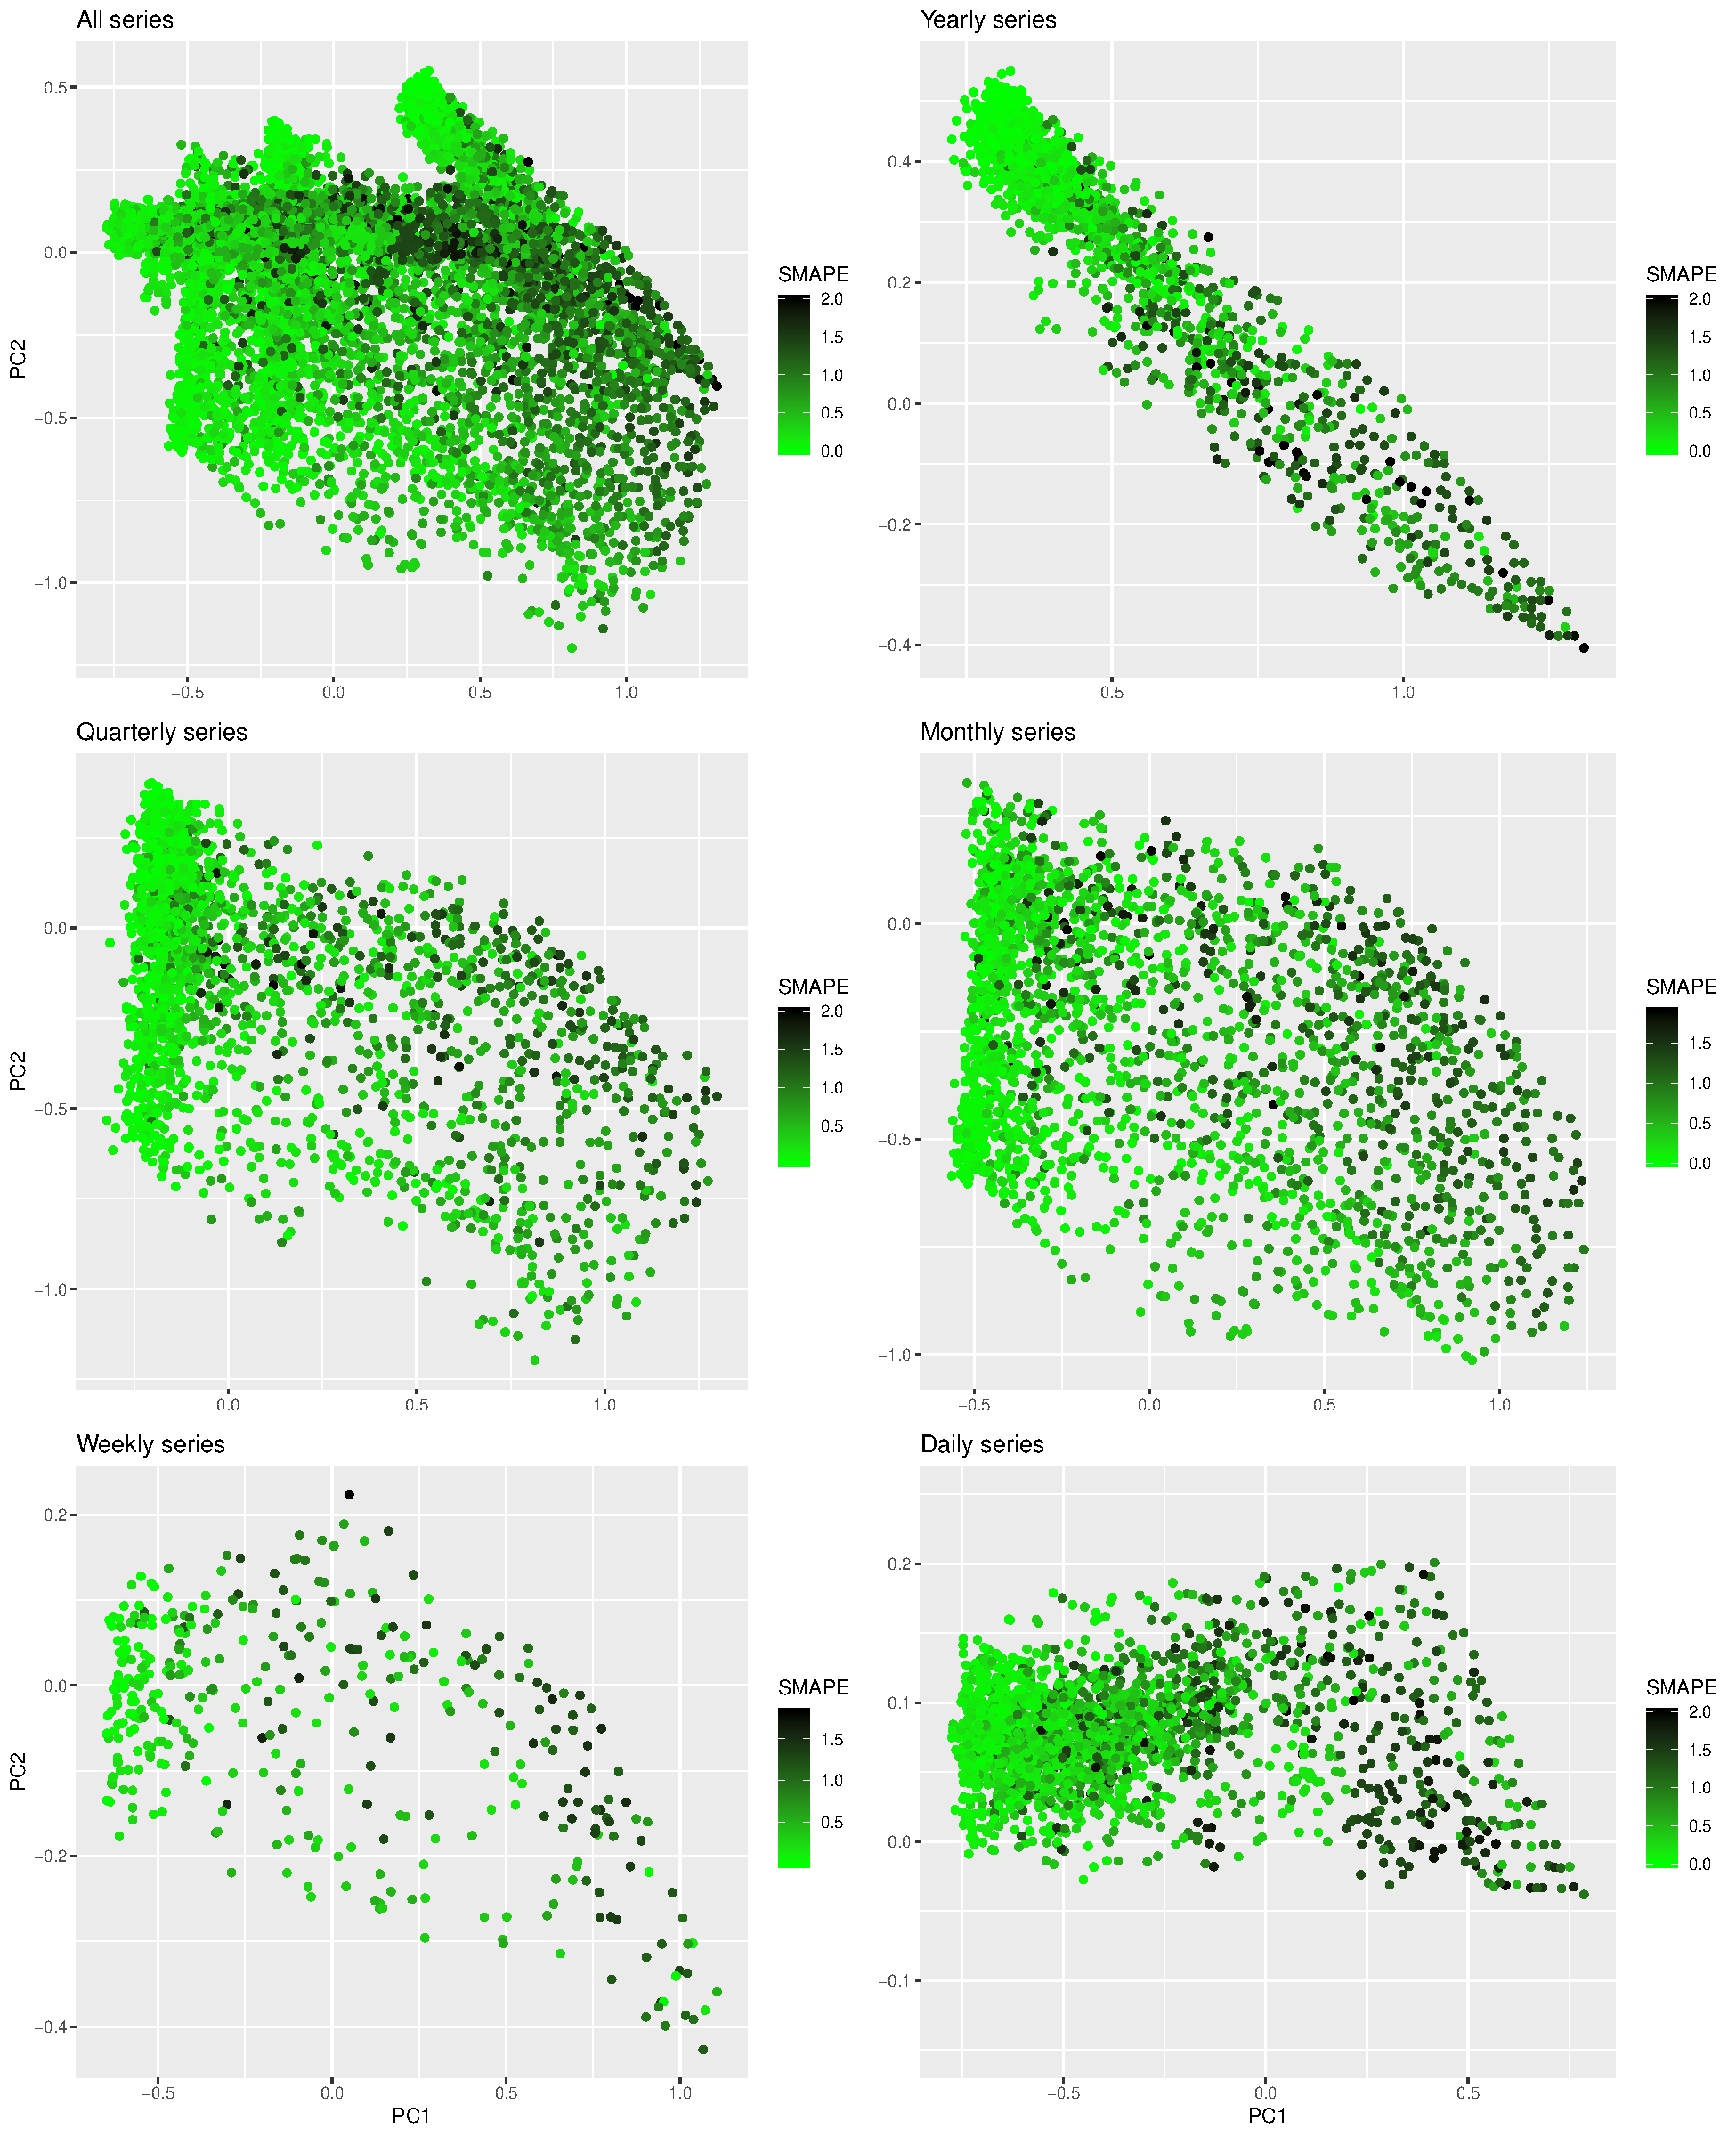
\includegraphics[width=
		\textwidth]{smape}%{./Pictures/mainscreen1.png}
	\end{center}
	
	
\end{figure} 
\end{document}
